\documentclass[12pt]{article} % Clase de documento
\usepackage[utf8]{inputenc}
\usepackage{csquotes} % Recommended for biblatex
\usepackage{tocbasic}  % Estilos de la TOC
\usepackage[spanish]{babel}
\usepackage{lmodern} % Soluciona problemas de sustitución de tamaño de fuente
\usepackage{amsfonts} % Para símbolos matemáticos
\usepackage{graphicx} % Para imágenes
\usepackage{hyperref} % Para enlaces y referencias en el índice
\usepackage{titling}  % Para personalizar la portada
\usepackage{geometry} % Márgenes
\usepackage{longtable}
\usepackage{multirow}
\usepackage{titlesec} % Para personalizar títulos
\usepackage{xcolor}
\usepackage[backend=bibtex,style=ieee]{biblatex}
\addbibresource{bibliografia.bib} % Archivo de bibliografía
\usepackage{amsmath} % Para ecuaciones matemáticas
\usepackage[T1]{fontenc}
\usepackage[table]{xcolor}
\usepackage{booktabs}
\usepackage{array}
\usepackage{rotating}
\usepackage{adjustbox}
\usepackage{makecell}
\usepackage{pdfpages}
% Personalización del título en la portada
\newcommand{\customtitlefont}{\fontsize{40pt}{42pt}\selectfont\bfseries} % Cambia el tamaño y estilo

\geometry{a4paper, margin=2.5cm}

\title{Detección de cáncer de mama a través de redes convolucionales}
\author{Marina Calero López \\
Lucas Manuel Herencia Solís \\
Juan Antonio Moreno Moguel \\
}
\date{\today}

\begin{document}
% PORTADA
\begin{titlepage}
    \centering
    {\customtitlefont \thetitle \par} % Título con tipografía personalizada
    \vspace{2cm}
    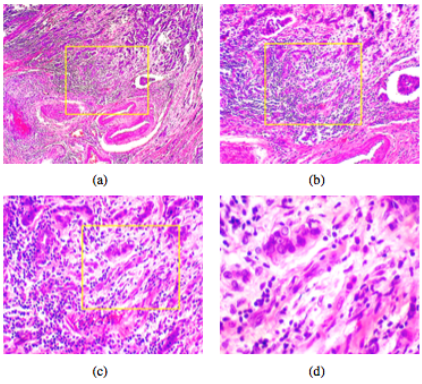
\includegraphics[width=0.8\textwidth]{logo.png}\par\vspace{1cm} % Imagen más grande
    {\scshape\Large Realizado por:\par}
    \vspace{1cm}
    {\Large \theauthor\par}
    \vfill
    {\large \thedate\par}
\end{titlepage}

% RESUMEN
\section*{Resumen}
Este proyecto se enmarca en la asignatura de Procesamiento de Imágenes Digitales (PID) y tiene como objetivo desarrollar un sistema que detecte el cáncer de mama mediante la identificación y comparación de células cancerígenas benignas y malignas. La metodología se basará en el uso de redes neuronales convolucionales (CNN) para analizar imágenes digitales de tejido mamario y extraer patrones característicos. Se realizan procesos de preprocesamiento, seguidos de la extracción de características específicas que permitan distinguir entre células malignas y benignas. Con este enfoque, se busca crear una herramienta de apoyo al diagnóstico clínico, que contribuya a una detección temprana y más precisa de la enfermedad. Además se realiza un estudio comparativo entre este enfoque y un enfoque más tradicional el cual aplica el clasificador K-Nearest Neighbours(KNN).


\vspace{.5cm}

\textbf{Palabras clave:} cáncer de mama, redes neuronales convolucionales (CNN), células, benigno, maligno.

\newpage
% ÍNDICE
\tableofcontents

\newpage

% CONTENIDO
\section{Introducción}
El cáncer de mama es una de las principales causas de mortalidad en el mundo, habiendo sido la responsable de 670.000 muertes en 2022 siendo a su vez el tipo de cáncer más común en las mujeres según el articulo \cite{who_breast_cancer}. Esto provoca que durante los últimos años se haya estado realizando una labor social enorme referente a la concienciación sobre el cáncer de mama dando gran importancia a su pronta detección.\\

\begin{figure}[!ht]
    \centering
    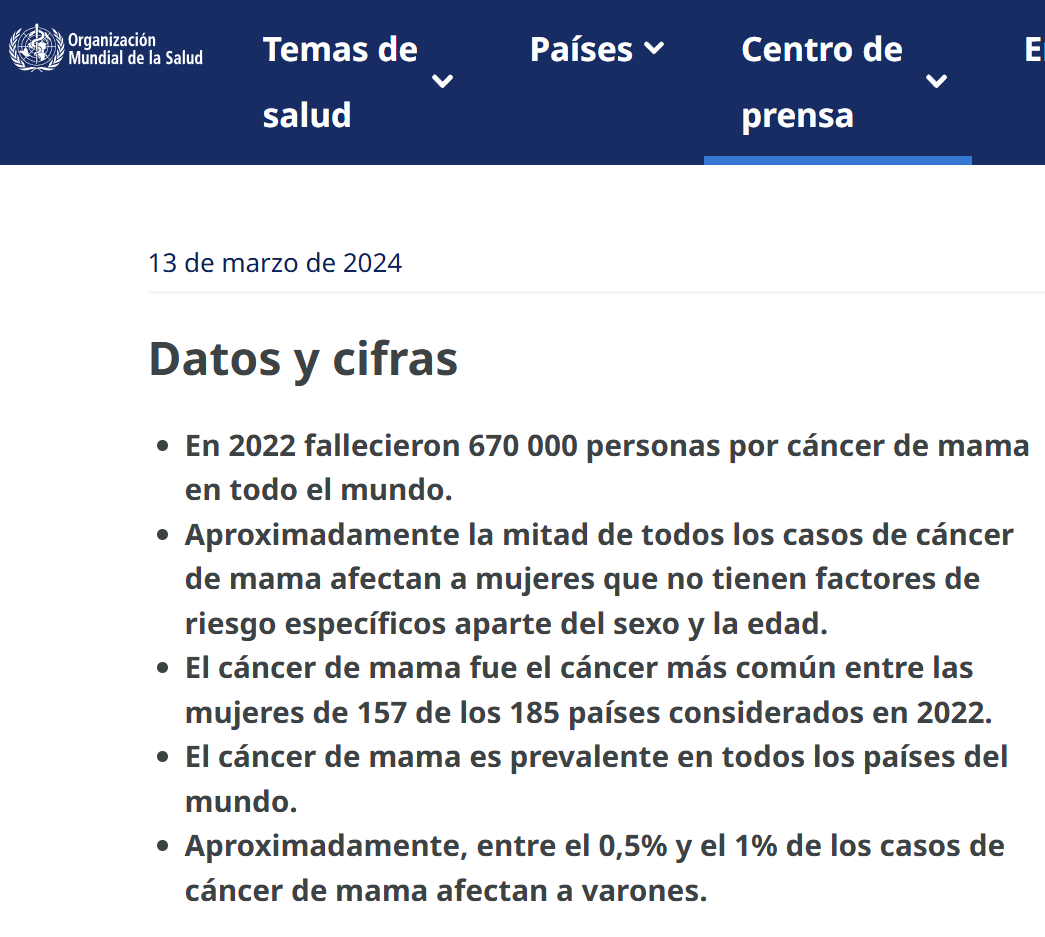
\includegraphics[width=0.49\textwidth]{introduccion.png}
    \caption{Cifras de la OMS \cite{who_breast_cancer}}
    \label{fig:OMS}
\end{figure}

Gracias a los avances en Deep Learning \cite{shinde2018review}, se han desarrollado métodos innovadores para analizar imágenes histológicas y detectar el cáncer de mama. En este contexto, se ha estudiado en el artículo científico \textit{\textbf{“Classification of breast cancer based on histology images using convolutional neural networks”}} \cite{bardou2018classification}, soportada por los 445 artículos en los que se realiza un estudio entre dos enfoques.\\

Con el objetivo de desarrollar una aplicación capaz de detectar cáncer de mama a partir de imágenes histológicas, utilizaremos dos enfoques distintos. El \textit{primer enfoque} se basa en una red neuronal convolucional (\textbf{CNN}), construida desde cero siguiendo la arquitectura del artículo principal \cite{bardou2018classification}, que permite realizar una clasificación directa de las imágenes entre tejido benigno y maligno. El \textit{segundo enfoque} emplea un modelo autoencoder convolucional preentrenado, obtenido desde un repositorio en línea, del cual se extrae la capa referente al encoder para la extracción de caraceterísticas de las imágenes. Esta representación comprimida de las imágenes, siendo un espacio latente de 48 dimensiones, se utiliza como entrada para el algoritmo K-Nearest Neighbors (\textbf{KNN}), que permite clasificar nuevas muestras en función de su similitud con otras ya conocidas.\\

Ambos métodos son implementados y evaluados con el objetivo de comparar su rendimiento, eficiencia y aplicabilidad dentro de un sistema de diagnóstico asistido por computadora. Esta comparación busca no solo medir la precisión, sino también explorar qué tipo de arquitectura resulta más adecuada para un entorno clínico real, donde la interpretabilidad, la escalabilidad y el tiempo de respuesta son factores clave.
\\
\section{Planteamiento del Teórico}
\subsection{Objetivos del Proyecto}

Este trabajo tiene como objetivo principal analizar y comparar diferentes metodologías de clasificación de imágenes médicas, con especial atención en la detección temprana del cáncer de mama. Para ello, se estudian dos enfonques, el primero mediante las CNN y el segundo mediante un modelo de autoencoder convolucional usando las KNN.\\

Los objetivos específicos del proyecto son los siguientes:\\

\begin{enumerate}
    \item \textbf{Crear} una aplicación que permita a los médicos detectar el cáncer de mama solo dando la imagen.
    \item \textbf{Desarrollar} los modelos que permitan la clasificación binaria de las imágenes.
    \item \textbf{Evaluar} el rendimiento de los modelos dependiendo de los pesos cargados según la amplitud de las imagenes evaluadas tanto para clasificación binaria tanto con CNN como KNN.
    \item \textbf{Realizar experimentación para análisis} del  impacto de las técnicas de aumento de datos sobre el desempeño de los modelos.
\end{enumerate}

\subsection{Tecnologías Utilizadas}
Para el desarrollo del proyecto se ha utilizado el lenguaje de programación \textbf{Python}\cite{python_org}, ampliamente adoptado en la comunidad científica por su simplicidad, legibilidad y amplio ecosistema de bibliotecas para el análisis de datos, visión por computador y aprendizaje automático.\\

El desarrollo de la interfaz de nuestra aplicación ha sido desarrollado utilizando \textbf{Tkinter}\cite{python_tkinter}, permitiendo de esta forma una selección y visualización de resultados cómoda de las imágenes junto a su clasificación en benigna o maligna.\\

Entre estas bibliotecas, se ha seleccionado \textbf{TensorFlow}\cite{tensorflow_org} como herramienta principal para la implementación y comparación de modelos. TensorFlow es una librería de código abierto desarrollada por Google que permite construir, entrenar y desplegar modelos de \textit{machine learning}, especialmente redes neuronales profundas. Su flexibilidad y eficiencia lo convierten en una plataforma ideal tanto para métodos tradicionales como para arquitecturas más complejas basadas en aprendizaje profundo.\\

\newpage
\subsection{Redes Neuronales Convolucionales (CNN)}
Una \textbf{Red Neuronal Convolucional} (CNN, por sus siglas en inglés) son una clase especializada de redes neuronales artificiales diseñadas para procesar datos con una estructura de tipo cuadrícula, siendo las imágenes un ejemplo típico. A diferencia de las redes neuronales tradicionales, las CNN son capaces de aprovechar la correlación espacial entre píxeles para identificar patrones jerárquicos, lo que las convierte en una herramienta sumamente eficaz en tareas de visión por computadora, análisis biomédico, reconocimiento de voz, entre otras aplicaciones.\\


\begin{figure}[!ht]
    \centering
    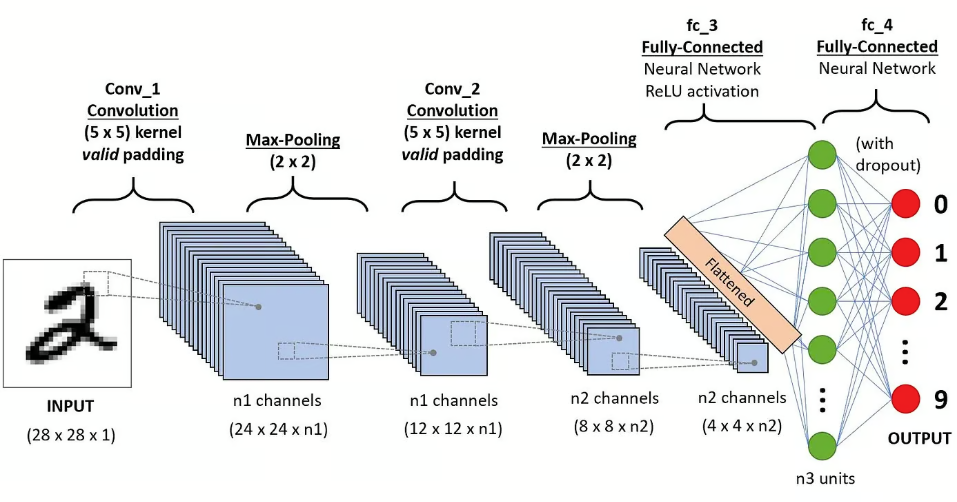
\includegraphics[width=0.65\textwidth]{CNN.png}
    \caption{Capas convolucionales \cite{datacamp_cnn}}
    \label{fig:capas_convolucionales}
\end{figure}
La arquitectura típica de una CNN está compuesta por una secuencia de capas que extraen representaciones abstractas de los datos de entrada. La primera etapa esencial en una CNN es la capa convolucional. Esta capa aplica filtros o \textit{“kernels”}, que recorren la imagen de entrada realizando una operación matemática denominada convolución. Cada filtro aprende a detectar características locales específicas, como formas, texturas o regiones de contraste. El resultado de esta operación es un conjunto de mapas de activación que reflejan la presencia de determinadas características en distintas regiones de la imagen \cite{lecun1998gradient}. \\

Tras la convolución, se aplica comúnmente una función de activación no lineal. La más utilizada en redes modernas es la función \textbf{ReLU} (Rectified Linear Unit), que introduce no linealidades en el modelo al anular los valores negativos. Esta operación permite a la red aprender representaciones más complejas que no podrían modelarse únicamente con funciones lineales \cite{nair2010rectified}. Sin embargo, una limitación conocida de ReLU es que, si las entradas son negativas, la función devuelve cero, lo que puede causar que algunas neuronas dejen de actualizarse durante el entrenamiento, un fenómeno conocido como el "\textit{problema de las neuronas muertas}". Para mitigar esta situación, se utiliza con frecuencia una variante llamada \textbf{Leaky ReLU}, la cual modifica la función para que permita un pequeño gradiente también en la región negativa. Matemáticamente, se define como: \[
\text{LeakyReLU}(x) = 
\begin{cases} 
x & \text{para } x > 0 \\
\alpha x & \text{para } x \le 0 
\end{cases}, \quad
\alpha = 0.01 \text{ (valor típico)}
\] Esta modificación mejora la capacidad de aprendizaje de la red al evitar que las neuronas queden inactivas de manera permanente \cite{maas2013rectifier}. \\

Posteriormente, se emplea una capa de agrupamiento, o pooling, que tiene como objetivo reducir la dimensionalidad espacial de los mapas de activación. Esta reducción permite disminuir el número de parámetros y operaciones computacionales, al tiempo que se mantiene la información más relevante. El agrupamiento también aporta robustez frente a pequeñas variaciones o distorsiones en la entrada \cite{sermanet2013overfeat}. \\

Las características extraídas a lo largo de las capas anteriores son finalmente procesadas por una o más capas completamente conectadas, también conocidas como \textit{fully connected layers}. En esta etapa, cada neurona está conectada a todas las salidas de la capa anterior, y la red combina las representaciones obtenidas para realizar una inferencia basada en el conocimiento aprendido. Esta parte del modelo funciona como un clasificador que transforma las representaciones espaciales en una predicción final.\\

La red concluye con una capa de salida que depende del tipo de problema que se desea resolver. En tareas de clasificación multiclase, se utiliza generalmente una función \textit{softmax} que devuelve una distribución de probabilidad sobre las clases. Para problemas de clasificación binaria, la función sigmoide es comúnmente empleada, ya que proporciona una probabilidad entre 0 y 1 que indica la pertenencia de la entrada a una de las dos clases posibles \cite{bishop2006pattern}.\\

El proceso de aprendizaje de una CNN se realiza mediante retropropagación, un algoritmo que ajusta los parámetros de la red a partir del error entre las predicciones y las etiquetas verdaderas. Este error se cuantifica mediante una función de pérdida, siendo la entropía cruzada una de las más utilizadas en problemas de clasificación. A su vez, algoritmos de optimización como Adam se encarga de actualizar los pesos del modelo en cada iteración, guiando el proceso de entrenamiento hacia una solución que minimice la pérdida \cite{kingma2014adam,rumelhart1986learning}. \\

En el apartado de Implementación se describe detalladamente cómo se ha construido la CNN usada.


\subsection{Autoencoder}
La estructura básica de un autoencoder consta de dos componentes principales (como muestra la Figura \ref{fig:autoencoder}): un codificador (\textbf{encoder}) y un decodificador (\textbf{decoder}). El \textbf{codificador} actúa de manera análoga a las primeras capas de una \textit{CNN}, tomando la entrada y transformándose progresivamente en una representación de menor dimensionalidad. Esta representación comprimida se denomina \textbf{espacio latente}, y constituye el núcleo informativo del autoencoder. Es en este espacio donde se concentran las características más relevantes de la entrada, de manera que, incluso tras eliminar redundancias o ruido, se retiene la información esencial \cite{bank2023autoencoders}. \\

En aplicaciones que integran CNN con autoencoders frecuentemente llamadas \textbf{convolutional autoencoders}, el codificador suele incluir capas convolucionales que permiten aprovechar las estructuras espaciales locales, de forma similar a una CNN estándar. Este diseño no solo reduce la dimensionalidad, sino que también conserva información espacial crítica para la reconstrucción posterior \cite{masci2011stacked}. \\

El \textbf{espacio latente} cumple una función crucial: actúa como un cuello de botella que obliga al modelo a aprender una codificación eficiente. A diferencia de una simple reducción de tamaño, esta compresión es aprendida automáticamente por la red en función de su capacidad para reconstruir los datos de entrada. Por esta razón, la calidad de la representación latente determina directamente el rendimiento del autoencoder. Si la codificación es adecuada, el decodificador será capaz de reconstruir la entrada con alta fidelidad, incluso cuando se utilice una representación mucho más compacta \cite{hinton2006reducing,goodfellow2016deep}. \\

El \textbf{decodificador}, por su parte, invierte el proceso realizado por el codificador. A partir del espacio latente, genera una reconstrucción de la entrada original utilizando capas que gradualmente expanden la dimensionalidad. En autoencoders convolucionales, esta expansión se realiza mediante \textbf{capas convolucionales transpuestas} o \textbf{upsampling}, que permiten reconstruir las estructuras espaciales originales. A diferencia del codificador, que se enfoca en extraer características, el decodificador se centra en aprender cómo esas características pueden combinarse para generar una salida coherente \cite{masci2011stacked}. \\

\begin{figure}[!ht]
    \centering
    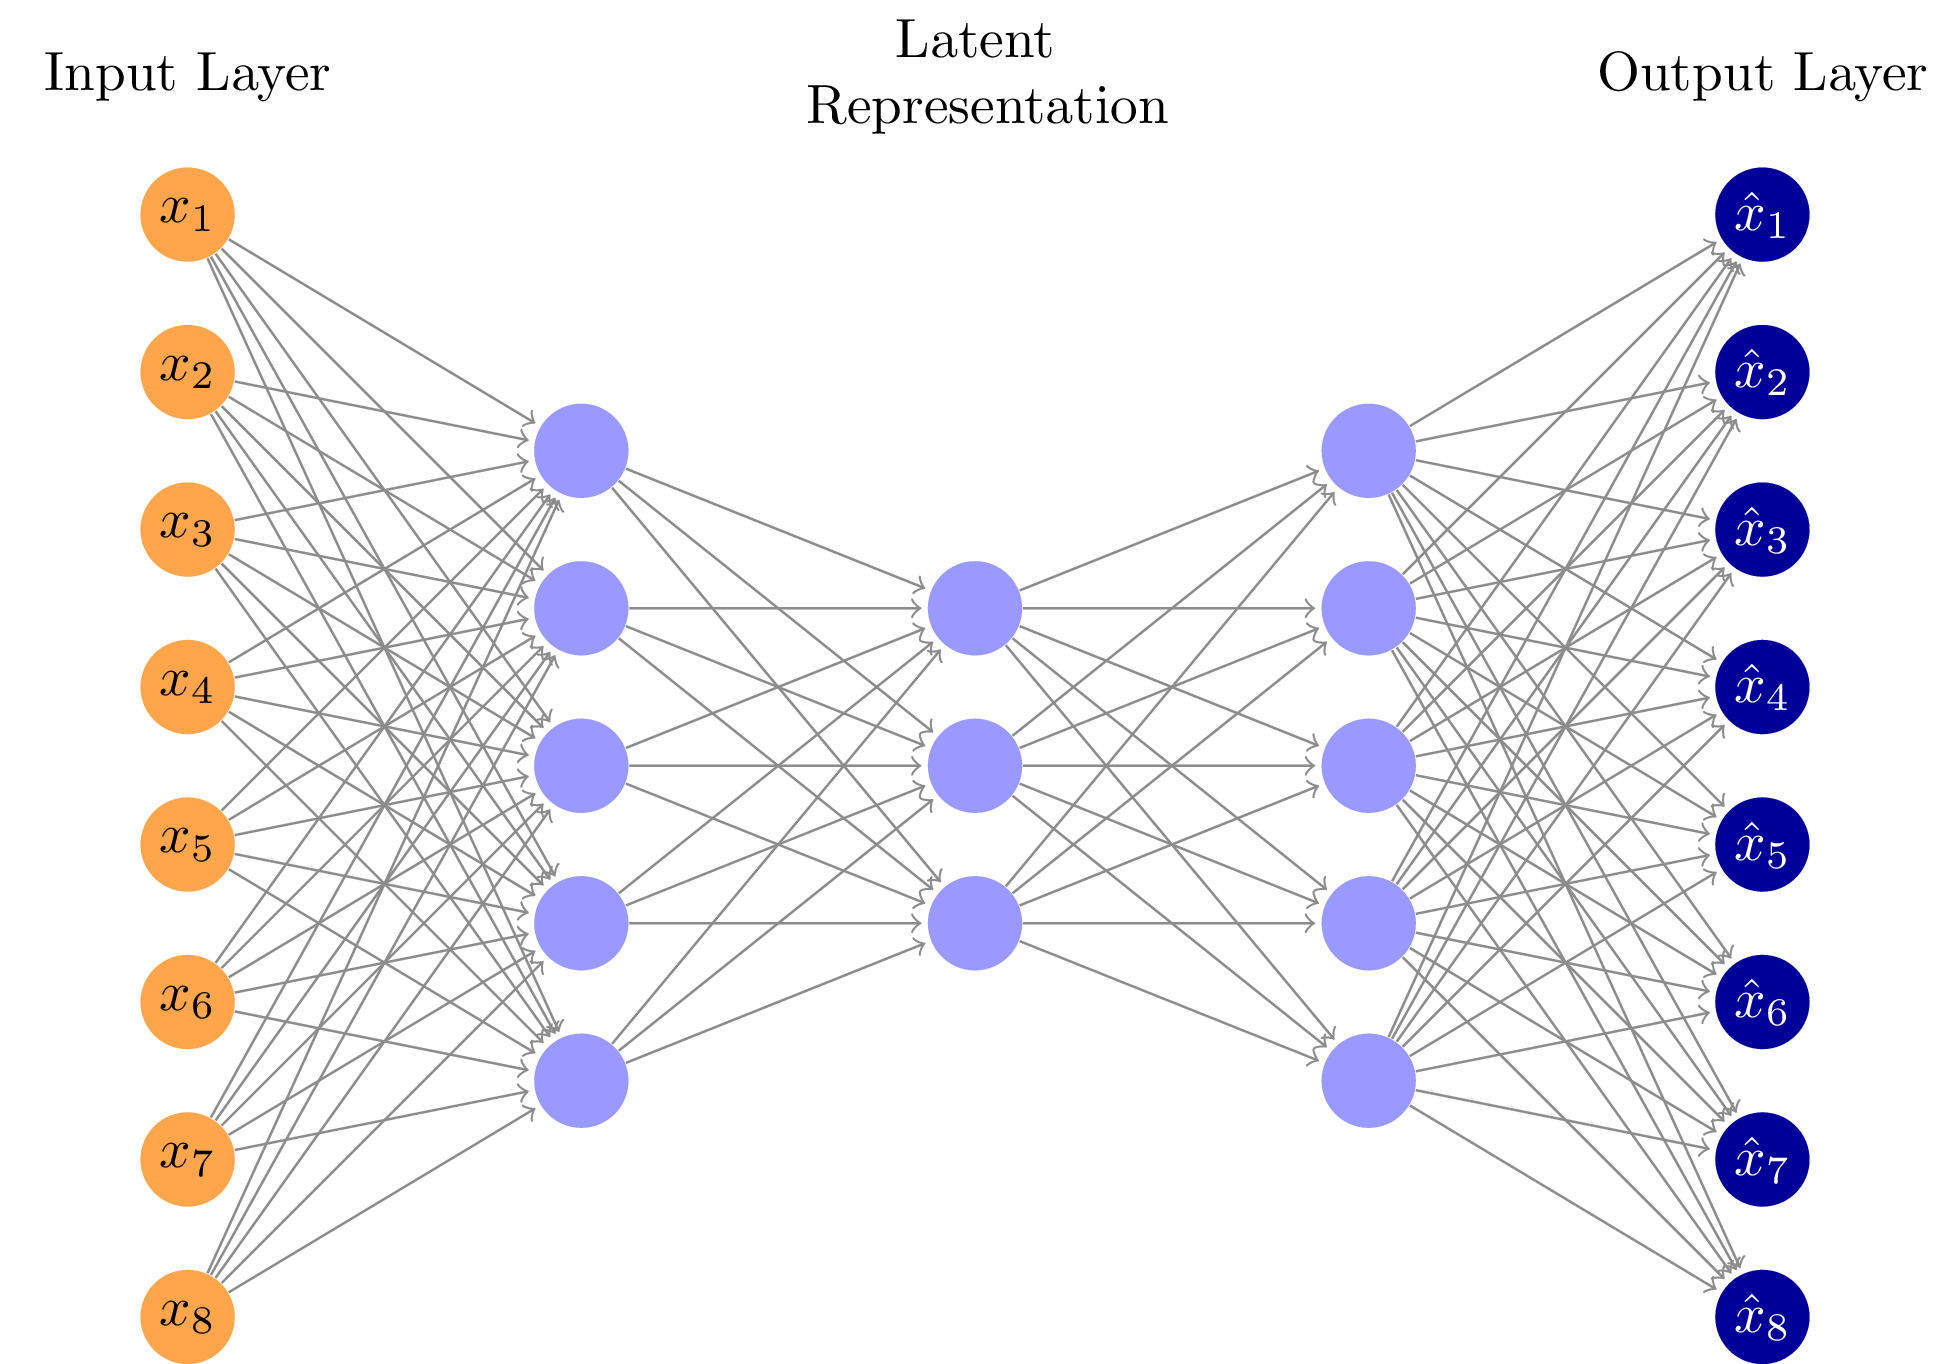
\includegraphics[width=0.9\textwidth]{autoencoder.png}
    \caption{Autoencoder\cite{janosh_autoencoder}}
    \label{fig:autoencoder}
\end{figure}

\subsection{K-Nearest Neighbours (KNN)}
El algoritmo \textbf{K-Nearest Neighbors} (KNN) es uno de los métodos más simples y efectivos dentro del aprendizaje automático supervisado. A diferencia de modelos como las redes neuronales, que requieren un proceso de entrenamiento explícito, el KNN es un método perezoso (\textit{lazy learner}), es decir, no construye un modelo a priori, sino que realiza la clasificación directamente a partir de los datos de entrenamiento disponibles \cite{cover1967nearest}. \\

La idea fundamental detrás del KNN es que una instancia se clasifica en función de las clases mayoritarias de sus \textbf{k vecinos más cercanos} en el espacio de características. Para determinar estos vecinos, se calcula la distancia entre la instancia a clasificar y cada punto del conjunto de entrenamiento, siendo la distancia euclidiana la medida más común, aunque otras como la distancia de Manhattan o la distancia de Mahalanobis también son utilizadas dependiendo del contexto del problema \cite{chomboon2015empirical}. \\

\begin{figure}[!ht]
    \centering
    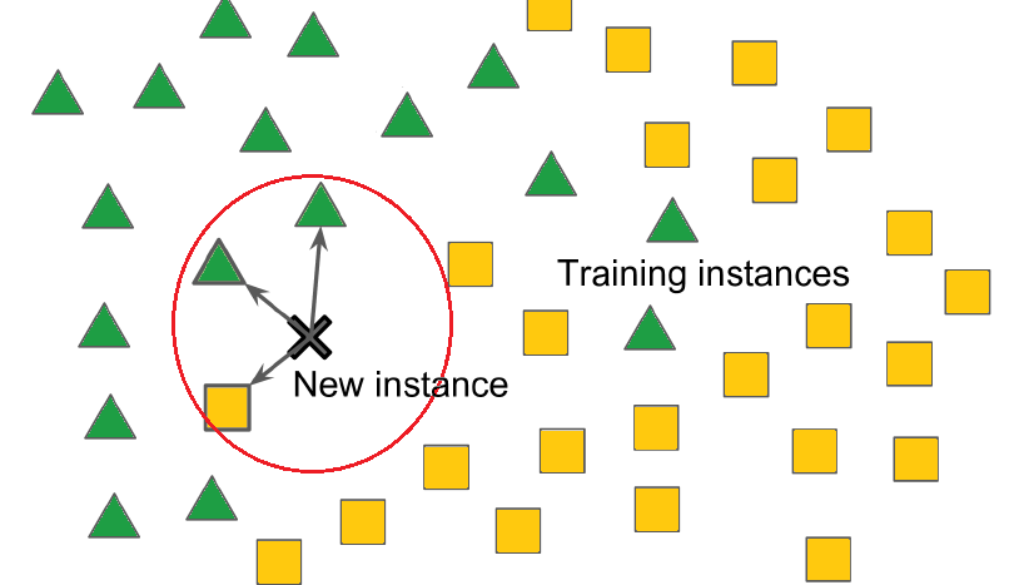
\includegraphics[width=0.8\textwidth]{knn.png}
    \caption{K-Nearest Neighbours \cite{mlarchive_knn}}
    \label{fig:knn}
\end{figure}

En el marco de arquitecturas más complejas como las \textbf{Redes Convolucionales} (CNN) o los autoencoders, el KNN se utiliza frecuentemente como clasificador final sobre las representaciones extraídas por estas redes. Por ejemplo, en lugar de utilizar capas completamente conectadas o \textit{softmax} para la \textbf{clasificación final}, es posible aplicar KNN sobre el \textbf{espacio latente} de un autoencoder o sobre los mapas de activación extraídos por las capas convolucionales. Esta estrategia es particularmente útil cuando se desea evaluar la \textbf{capacidad discriminativa de la representación aprendida}, independiente de la arquitectura del clasificador \cite{van2009dimensionality}. \\

Una de las principales ventajas del KNN en estos contextos es su \textbf{robustez} y \textbf{simplicidad}. No requiere entrenamiento adicional una vez se ha obtenido la representación latente, y su rendimiento depende únicamente de la calidad del espacio de características. Esto lo convierte en una herramienta ideal para comparar distintas representaciones, realizar pruebas rápidas sin necesidad de reentrenar redes profunda \cite{bengio2013representation}. \\

Sin embargo, KNN también presenta limitaciones. Su eficiencia computacional disminuye cuando el número de muestras o la dimensionalidad del espacio de características es muy alta, este es un problema conocido como la "\textit{maldición de la dimensionalidad}". Por ello, su uso suele estar precedido por una etapa de reducción de dimensionalidad o extracción de características, como las proporcionadas por autoencoders o CNN, que ayudan a preservar solo la información más relevante \cite{aggarwal2014data}. \\

\newpage
\section{Implementación}
El desarrollo de este proyecto se fundamenta en el uso de técnicas de aprendizaje automático y profundo para la clasificación de imágenes histológicas de cáncer de mama. Con el objetivo de comparar el rendimiento entre distintos enfoques, se han implementado y entrenado dos tipos de modelos: el primero, una CNN, y el segundo, la capa de encoder extraida de un autoencoder y usando después un clasificador KNN para obtener el resultado. Ambos modelos han sido entrenados utilizando un conjunto de imágenes histológicas públicamente disponibles.\\

\subsection{Descripción del dataset}
Para el desarrollo de este proyecto se utilizó el \textbf{dataset de imágenes histológicas de cáncer de mama BreaKHis} \cite{google_drive_folder}, asociado al trabajo \cite{bardou2018classification}, ampliamente reconocido en la literatura científica por su utilidad en investigaciones de diagnóstico asistido por computadora en cáncer de mama. Este dataset contiene un total de 9,109 imágenes histopatológicas de tejido tumoral mamario, recolectadas de 82 pacientes en el artículo \cite{spanhol2015dataset}.\\

Las muestras se obtuvieron mediante biopsia excisional (\textbf{SOB}), también conocida como mastectomía parcial, un procedimiento quirúrgico realizado bajo anestesia general que permite extraer una porción significativa de tejido para su análisis. Las imágenes fueron teñidas con hematoxilina y eosina (H\&E), y capturadas mediante un microscopio óptico en cuatro niveles de aumento: 40X, 100X, 200X y 400X. Todas las imágenes presentan una resolución de 700×460 píxeles, están en formato PNG, y utilizan un modelo de color RGB de 3 canales. \\

BreaKHis está dividido en dos clases principales: tumores \textbf{benignos} (2,480 imágenes) y tumores \textbf{malignos} (5,429 imágenes). Cada una de estas clases se subdivide en cuatro tipos histológicos distintos, basados en la morfología observada al microscopio: \\

\begin{itemize}
    \item \textbf{Benignos:} Adenosis (A), Fibroadenoma (F), Tumor filoides (PT) y Adenoma tubular (TA).
    \item \textbf{Malignos:} Carcinoma ductal (DC), Carcinoma lobulillar (LC), Carcinoma mucinoso (MC) y Carcinoma papilar (PC).
\end{itemize}

En esta investigación se utilizó una versión del dataset disponible públicamente \cite{google_drive_folder}, la cual se encuentra organizada de forma estructurada para entrenamiento, validación y evaluación, dividiéndose a su vez en magnificación y tipo, lo que facilitó la gestión y preparación de los datos para el entrenamiento de los modelos. \\

\subsection{Arquitectura de la aplicación}
Esta aplicación de escritorio ha sido desarrollada con Python utilizando la biblioteca \textbf{Tkinter} y la extensión \textbf{tkinterdnd2} para soporte de arrastrar y soltar. Está diseñada para facilitar el análisis automatizado de imágenes microscópicas de tejidos mamarios, permitiendo la clasificación entre lesiones benignas y malignas mediante modelos de machine learning. La interfaz ofrece una experiencia visual amigable y funcional para profesionales o investigadores del área médica.\\

\textbf{Principales funcionalidades:} 

\begin{enumerate}
    \item \textbf{Carga de imágenes eficiente:}  Permite seleccionar múltiples imágenes desde el sistema de archivos o mediante arrastrar y soltar directamente sobre el área de previsualización. Soporta formatos como PNG, JPG, JPEG, BMP y GIF.

    \item \textbf{Previsualización y navegación:} Muestra una imagen ampliada de la muestra seleccionada y un carrete con miniaturas generadas automáticamente, facilitando la revisión manual. Se utiliza \textcolor[HTML]{006400}{\texttt{PIL.Image}} para procesar imágenes y \textcolor[HTML]{006400}{\texttt{ImageTk.PhotoImage}} para su integración en la GUI.
    \item \textbf{Selector de modelo de análisis:} Incluye un desplegable con modelos disponibles: KNN y CNN, con variantes según niveles de aumento (40x, 100x, 200x, 400x), permitiendo seleccionar el tipo de entrenamiento más adecuado según la resolución de las imágenes, además de una sección experimental para cada modelo en la que se tomo del entrenamiento con mezcla todos los aumentos como entrada.
    \item \textbf{Ejecución y control del análisis:} 
    Los análisis se realizan de forma secuencial mediante hilos (\textcolor[HTML]{006400}{\texttt{threading.Thread}}) para mantener la interfaz fluida. Los modelos son invocados a través de funciones importadas desde los módulos \textcolor[HTML]{006400}{\texttt{knn.py}} y \textcolor[HTML]{006400}{\texttt{cnn.py}}, que devuelven una predicción y un color representativo.
    \item \textbf{Visualización de resultados y estadísticas:}
    Para cada imagen se muestra el resultado (Benigno/Maligno) con retroalimentación visual (círculo coloreado) y se actualizan las estadísticas globales: cantidad total de imágenes, benignas y malignas. Se incluye también una barra de progreso (\textcolor[HTML]{006400}{\texttt{ttk.Progressbar}}).
    \item \textbf{Gestión del análisis:} 
    Se ofrecen botones para iniciar, pausar/reanudar y eliminar las imágenes seleccionadas. Los resultados se limpian automáticamente al cargar nuevas imágenes o al reiniciar el análisis.
\end{enumerate}

\subsection{Arquitectura CNN}
Para la implementación del modelo CNN se ha seguido la arquitectura descrita en el artículo \textbf{“\textit{Classification of Breast Cancer Based on Histology Images Using Convolutional Neural Networks}”} \cite{bardou2018classification}, en el cual se desarrolla una red neuronal convolucional (CNN) especialmente diseñada para abordar el desafío de clasificar imágenes histológicas de tejido mamario teñidas con hematoxilina y eosina (H\&E).\\

El modelo desarrollado presenta una estructura jerárquica compuesta por \textit{5 capas convolucionales}, seguidas de dos capas completamente conectadas y una capa de salida con activación \textit{softmax}. Cada capa convolucional aplica filtros (también denominados \textit{kernels}) de tamaño 3×3, que se deslizan sobre la imagen para detectar patrones locales como bordes, texturas o regiones celulares características. En detalle, la \textit{primera} capa genera 64 mapas de características; la \textit{segunda}, 96; la \textit{tercera}, 128; y tanto la \textit{cuarta} como la \textit{quinta}, 256 mapas. Estas capas permiten una extracción progresiva de características, pasando de representaciones simples a otras más abstractas y complejas.\\

Tras las capas convolucionales, se emplean operaciones de \textbf{max pooling} en la primera, segunda y quinta capa, utilizando ventanas de 3×3 con un stride de 2. El \textit{max pooling} selecciona el valor máximo dentro de cada región, reduciendo así la resolución espacial de las representaciones internas y proporcionando invariancia ante pequeñas traslaciones. El \textit{stride}, o paso de desplazamiento, controla cuántos píxeles se avanza al aplicar esta operación; un valor de 2 reduce la dimensionalidad de forma más agresiva. Las capas tercera y cuarta no aplican \textit{pooling}, lo cual permite conservar la resolución espacial de las características extraídas, favoreciendo una mayor sensibilidad a detalles finos del tejido. \\

Todas las capas convolucionales están seguidas por una función de activación ReLU \texttt{(Rectified Linear Unit)}, definida como: \begin{equation} f(x) = \max(0, x) \end{equation}, que introduce no linealidad en el modelo y mejora la eficiencia del entrenamiento al evitar el problema del desvanecimiento del gradiente. Los pesos de estas capas se inicializan a partir de una distribución normal con desviación estándar pequeña ($0.01$), y se aplica regularización L2 (\textit{weight decay}) con un coeficiente de penalización de $\lambda = 10^{-3}$, lo cual ayuda a evitar el sobreajuste penalizando los pesos excesivamente grandes.\\

A la salida de las capas convolucionales, los mapas de activación se aplanan mediante una capa \textit{Flatten}, que convierte las matrices tridimensionales en un vector unidimensional para conectarlas con las capas densas. La primera capa densa contiene 2000 neuronas con activación ReLU y se acompaña de una capa \textit{Dropout} con una probabilidad de desactivación del 50\%. Esta técnica consiste en \textit{“apagar”} aleatoriamente la mitad de las neuronas durante el entrenamiento, reduciendo así la dependencia entre unidades y mejorando la capacidad de generalización del modelo. Finalmente, la segunda capa densa contiene tantas neuronas como clases en el problema (en este caso, dos) y emplea una activación \textit{softmax}, que convierte las salidas en una distribución de probabilidad sobre las clases, facilitando la clasificación final.\\

Finalmente, el modelo puede entrenarse sobre imágenes con distintas magnificaciones o bien utilizando un conjunto combinado, y se proporciona la funcionalidad para guardar tanto el modelo completo como únicamente los pesos aprendidos. Esta flexibilidad resulta útil tanto para entrenamientos posteriores como para su integración en entornos clínicos.\\

Al finalizar el proceso de entrenamiento, se generan a partir del mismo modelo 5 archivos con los pesos obtenidos tras el entrenamiento, cada uno de estos se ha entrenado con un conjunto de datos distintos, ya sea utilizando la totalidad de los datos disponibles o únicamente aquellos correspondientes a una de las magnificaciones específicas: 40X, 100X, 200X o 400X. 

\subsection{Arquitectura KNN}
Se emplea un autoencoder convolucional basado en el artículo \cite{minarno2021cnn} para la recuperación de imágenes histológicas de cáncer de mama. Este modelo, compuesto por un codificador y un decodificador, extrae representaciones latentes útiles para clasificación o búsqueda por similitud. Se entrena minimizando el error de reconstrucción mediante optimizadores como Adam, utilizando conjuntos de entrenamiento. Este tipo de red se caracteriza por una estructura simétrica compuesta por dos partes principales: el codificador y el decodificador.. \\

\begin{enumerate}
    \item \textbf{Codificación (Encoder):} cse encarga de transformar la imagen de entrada en una representación latente de baja dimensionalidad mediante una serie de capas convolucionales con filtros de tamaño 3×3 y funciones de activación ReLU. Estas capas están acompañadas por operaciones de max pooling que reducen progresivamente la resolución espacial, extrayendo características jerárquicas de alto nivel. El resultado es un vector latente de \textbf{48 dimensiones}, correspondiente al cuello de botella del modelo, que encapsula la información visual más relevante de la imagen.
    \item \textbf{Decodificación (Decoder):} intenta reconstruir la imagen original a partir de esta representación comprimida, utilizando capas de upsampling y convolucionales dispuestas simétricamente respecto al codificador. El entrenamiento del autoencoder se realiza minimizando el error cuadrático medio (MSE) entre la imagen de entrada y su reconstrucción, obligando así al modelo a aprender una codificación eficiente y significativa.
\end{enumerate}

Tras el proceso de extracción de características mediante el autoencoder convolucional gracias a su capa de encoder, cada imagen del conjunto de datos es transformada en un vector latente de 48 dimensiones, que representa las características más relevantes de la imagen histológica en un espacio comprimido. Estos vectores latentes, junto con su etiqueta de clase correspondiente (por ejemplo, benigno o maligno), se almacenan en un archivo \textbf{JSON} que actúa como base de datos para el sistema de clasificación.\\

Para realizar la clasificación de una nueva imagen, se sigue el siguiente procedimiento:

\begin{enumerate}
    \item \textbf{Extracción del vector latente:} La imagen de entrada se procesa a través del codificador previamente entrenado, extrayendo su correspondiente vector de características.
    
    \item \textbf{Cálculo de distancias:} Se calcula la \textbf{distancia euclidiana} entre este vector y todos los vectores almacenados en el conjunto indexado. La distancia euclídea entre dos vectores \( x \) e \( y \) se define como:
    
    \begin{equation}
        d(x, y) = \sqrt{ \sum_{i=1} (x_i - y_i)^2 }
    \end{equation}

    \item \textbf{Selección de los vecinos más cercanos:} Una vez calculadas todas las distancias, se seleccionan los \textbf{k vectores más cercanos}, siendo \(k \)= 5 en esta implementación. Estos representan las imágenes más similares en el espacio latente.
    \item \textbf{Clasificación por mayoría:} Se toma la clase más común entre los cinco vectores más próximos, y esta se asigna como la \textbf{predicción final} para la imagen de entrada.

\end{enumerate}

Este enfoque no requiere un entrenamiento explícito del clasificador, ya que el método KNN funciona de forma \textbf{perezosa} (lazy learning) y opera directamente sobre las instancias almacenadas. Gracias a la alta calidad de las características extraídas por el autoencoder, el sistema logra clasificaciones precisas sin necesidad de arquitecturas más complejas.

\subsection{Evaluación del Sistema}
Los modelos fueron evaluados mediante un conjunto de métricas de clasificación binaria, entendiendo que los benignos serán los casos negativos y los malignos los casos positivos:

\begin{enumerate}
    \item \textbf{Precisión (accuracy):} mide la proporción de predicciones correctas respecto al total de muestras evaluadas. Se calcula como:
    \begin{equation}
        \text{accuracy} = \frac{VP + VN}{VP + VN + FP + FN}
    \end{equation}
    
    \item \textbf{Sensibilidad (recall):} evalúa la capacidad del modelo para identificar correctamente las muestras positivas. Se calcula como:
    \begin{equation}
        \text{recall} = \frac{VP}{VP + FN}
    \end{equation}
    
    \item \textbf{Precisión (precision):} cuantifica la proporción de muestras clasificadas como positivas que realmente lo son. Se calcula como:
    \begin{equation}
        \text{precision} = \frac{VP}{VP + FP}
    \end{equation}
    
    \item \textbf{F1 Score:} proporciona una medida balanceada entre la precisión y la sensibilidad, siendo especialmente útil en contextos donde existe un desequilibrio entre clases. Se calcula como:
    \begin{equation}
        F1 = 2 \cdot \frac{\text{precision} \cdot \text{recall}}{\text{precision} + \text{recall}}
    \end{equation}
\end{enumerate}



Estas métricas fueron calculadas de forma individual para cada uno de los modelos entrenados, lo que permitió realizar un análisis cuantitativo del impacto que tiene el tipo de arquitectura como \textit{K-Nearest Neighbors} (KNN) y \textit{Convolutional Neural Networks} (CNN) sobre el rendimiento en la tarea de clasificación. \\

Adicionalmente, se evaluó la influencia de distintos niveles de \textit{data augmentation} aplicados a las imágenes de entrada, tanto para KNN como con CNN con el fin de observar cómo afectan la capacidad de generalización de los modelos.\\

Como parte del trabajo, se llevó a cabo una experimentación adicional orientada a evaluar el impacto de una integración más profunda entre los enfoques basados en KNN y CNN. En esta etapa, se creó un sistema de almacenamiento que registró todas las representaciones extraídas de las imágenes mediante el modelo KNN, sin restricciones en cuanto a la dimensión o amplitud de dichas características. Paralelamente, se entrenó un modelo CNN utilizando la totalidad del conjunto de imágenes disponibles, y se extrajeron los pesos resultantes tras el entrenamiento completo del modelo. Esta experimentación se realizó con el fin de observar qué resultados podían obtenerse al disponer de ambas fuentes de representación, y explorar su posible utilidad en tareas de clasificación médica. 

 

\section{Experimentación}
Para llevar a cabo la experimentación, se realizaron pruebas sobre un conjunto de datos al que se le aplicará \textit{data augmentation} con el objetivo de evaluar la robustez y capacidad de generalización de los modelos. Las técnicas de aumento de datos incluirán transformaciones como rotaciones de un rango entre $-30^\circ$ a $30^\circ$ y modificaciones en la intensidad de las imágenes, con un factor de entre $0.7$ (oscurece) a $1.3$ (ilumina), simulando variaciones realistas que podrían encontrarse en escenarios del mundo real. Esto permitirá analizar cómo afecta la variabilidad de entrada al rendimiento de los modelos evaluados. \\

En esta etapa, se llevará a cabo una comparación de rendimiento entre dos enfoques de clasificación: una red neuronal convolucional (\textit{CNN}) entrenada sobre cada variedad de las imágenes aumentadas y un entrenamiento con todas las imágenes en global, y un modelo \textit{K-Nearest Neighbors} (\textit{KNN}) diseñado de forma personalizada para cada uno de las posibles variaciones de imágenes respecto a su aumento. Esta comparación permitirá observar las diferencias entre un enfoque basado en aprendizaje profundo y otro basado en métodos clásicos de aprendizaje supervisado, en cuanto a métricas de \textit{accuracy}, \textit{precisión}, \textit{recall} y \textit{F1-score}.

A continuación se muestran los resultados de las pruebas realizadas para entender de mejor manera la robustez y adaptabilidad de los distintos modelos:

\begin{figure}[!ht]
    \centering
    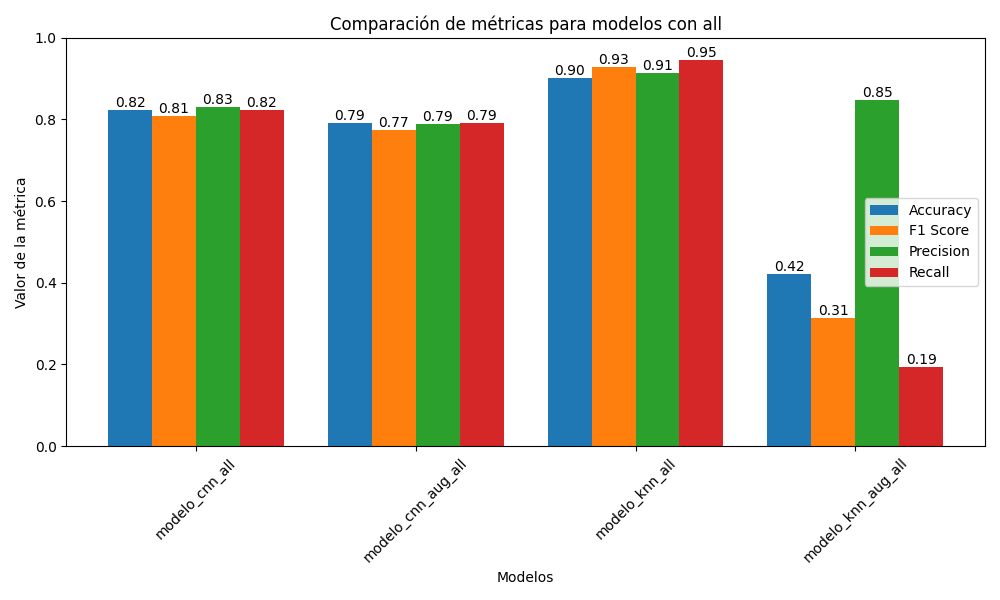
\includegraphics[width=0.7\textwidth]{comparison_all.png}
    \caption{Métrica para CNN y KNN al ser probados con el dataset completo y con el dataset aumentado.}
    \label{fig:figura1}
\end{figure}

\newpage
\begin{figure}[!ht]
    \centering
    \begin{minipage}[b]{0.45\textwidth}
        \centering
        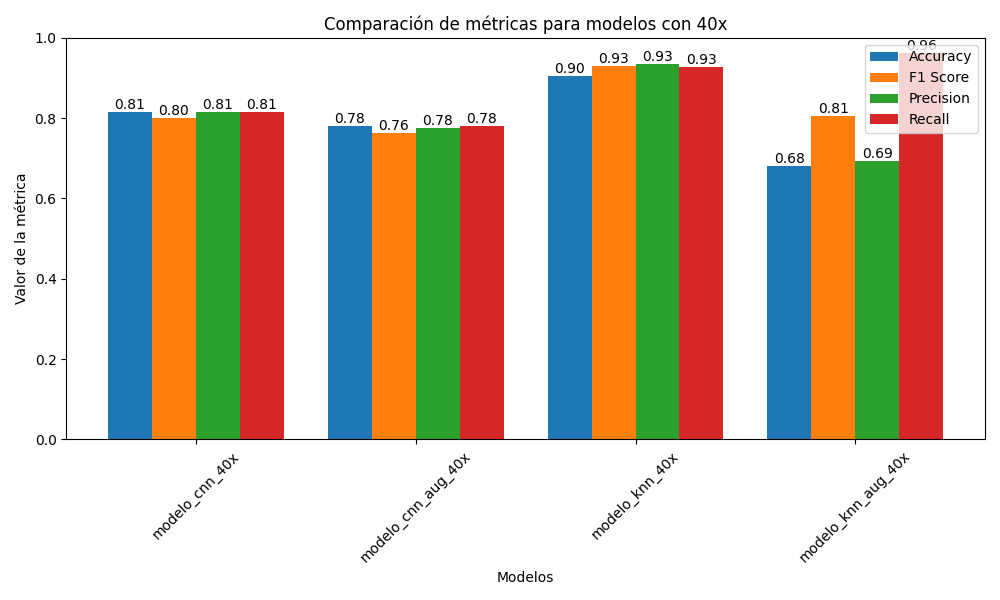
\includegraphics[width=\textwidth]{comparison_40x.png}
        \caption{Métrica para CNN y KNN al ser probados con el dataset de 40X y con el dataset aumentado.}
        \label{fig:figura2}
    \end{minipage}
    \hfill
    \begin{minipage}[b]{0.45\textwidth}
        \centering
        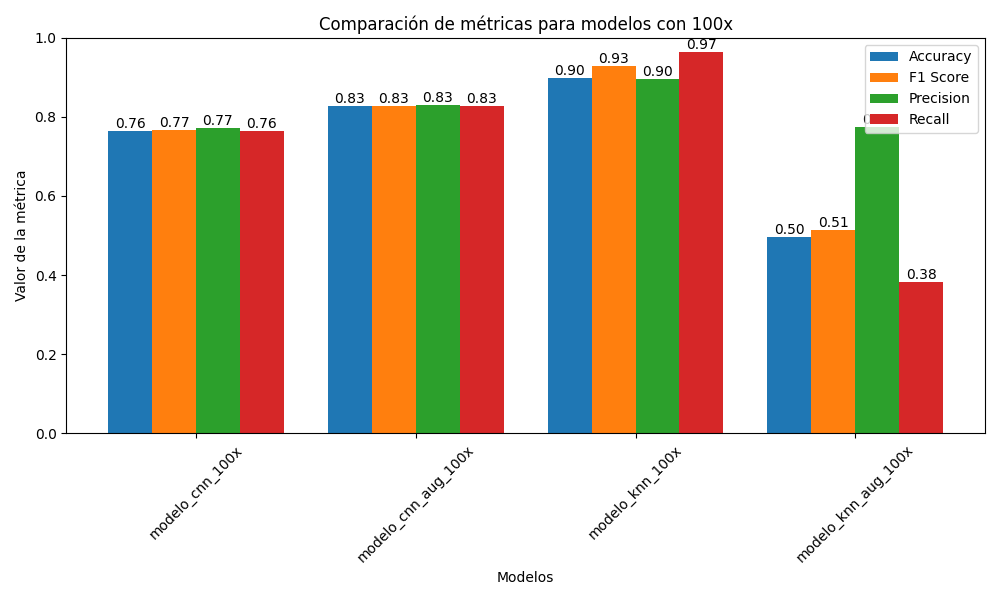
\includegraphics[width=\textwidth]{comparison_100x.png}
        \caption{Métrica para CNN y KNN al ser probados con el dataset de 100X y con el dataset aumentado.}
        \label{fig:figura3}
    \end{minipage}
    \vspace{0.5cm}
    \begin{minipage}[b]{0.45\textwidth}
        \centering
        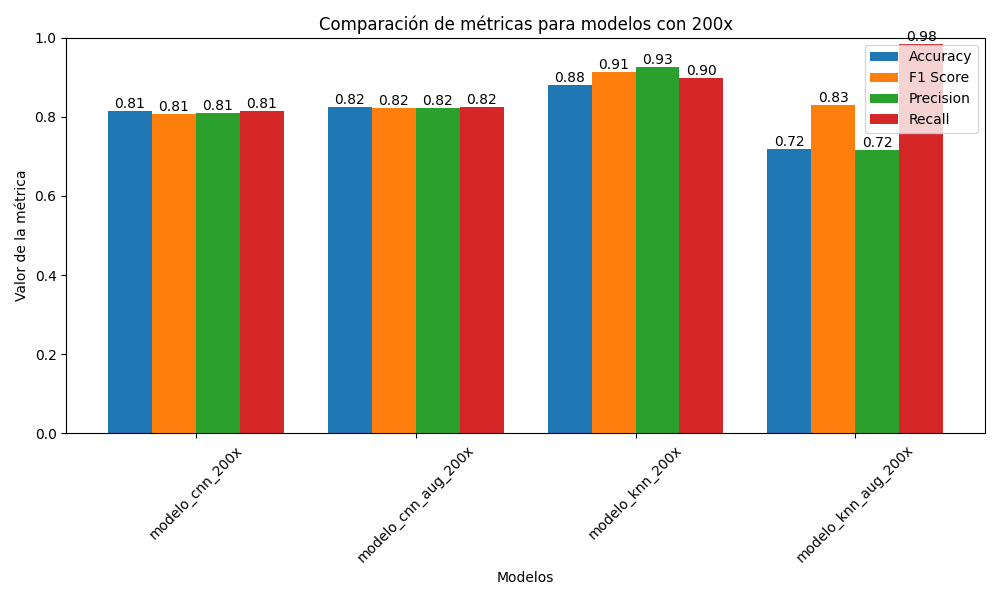
\includegraphics[width=\textwidth]{comparison_200x.png}
        \caption{Métrica para CNN y KNN al ser probados con el dataset de 200X y con el dataset aumentado.}
        \label{fig:figura4}
    \end{minipage}
    \hfill
    \begin{minipage}[b]{0.45\textwidth}
        \centering
        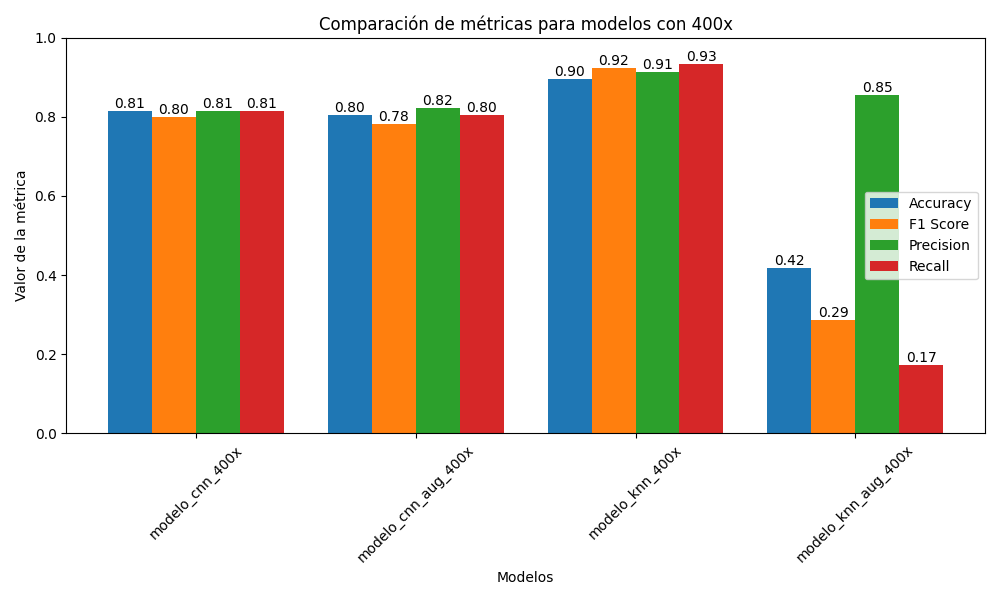
\includegraphics[width=\textwidth]{comparison_400x.png}
        \caption{Métrica para CNN y KNN al ser probados con el dataset de 400X y con el dataset aumentado.}
        \label{fig:figura5}
    \end{minipage}
    \hfill
    \begin{minipage}[b]{0.45\textwidth}
        \centering
        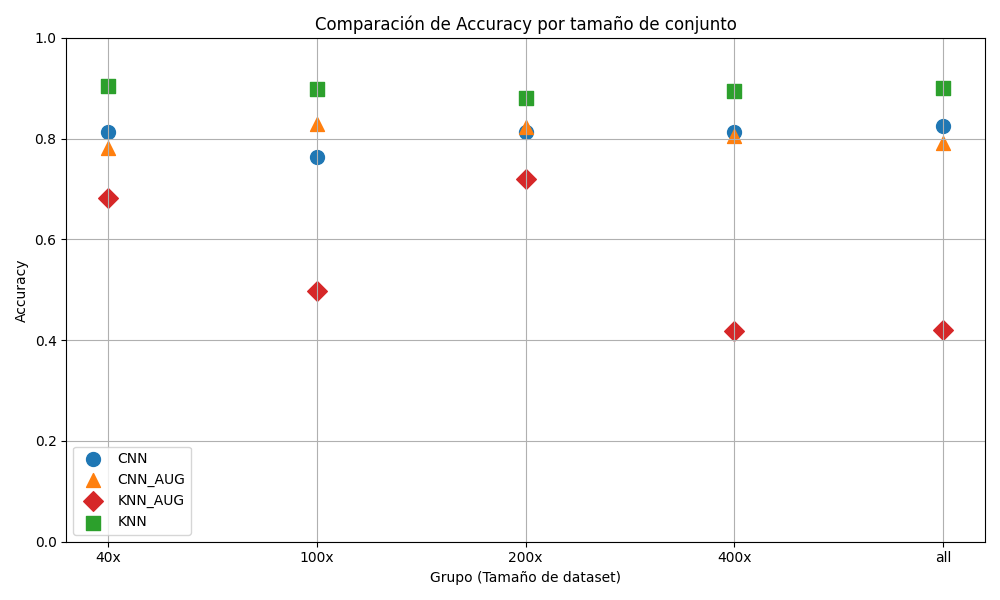
\includegraphics[width=\textwidth]{accuracy_comparativa_puntos.png}
        \caption{Comparación de accuracy}
        \label{fig:figura6}
    \end{minipage}
    \hfill
    \begin{minipage}[b]{0.45\textwidth}
        \centering
        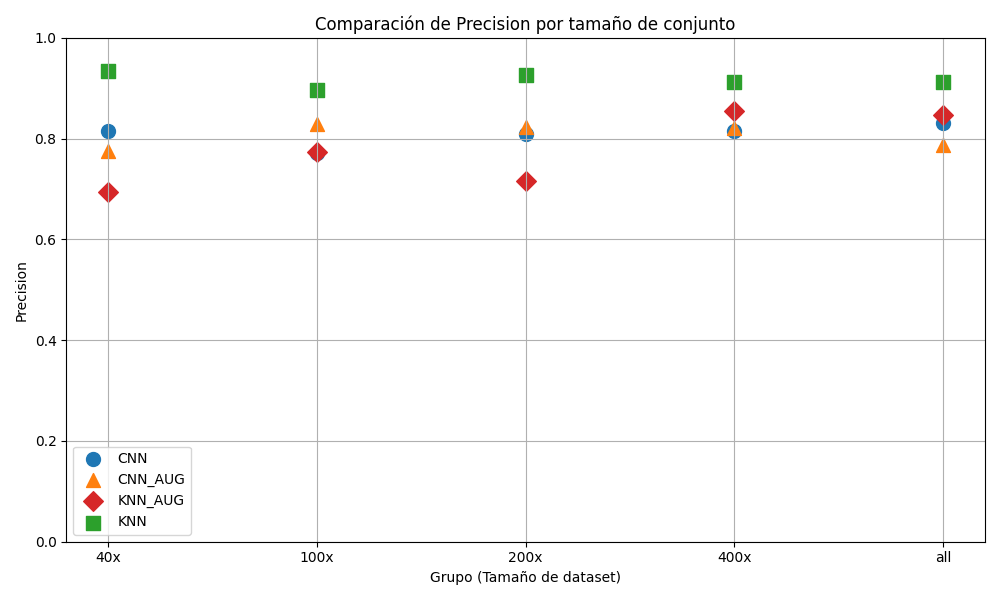
\includegraphics[width=\textwidth]{precision_comparativa_puntos.png}
        \caption{Comparación de precision}
        \label{fig:figura7}
    \end{minipage}
    \vspace{0.5cm}
    \begin{minipage}[b]{0.45\textwidth}
        \centering
        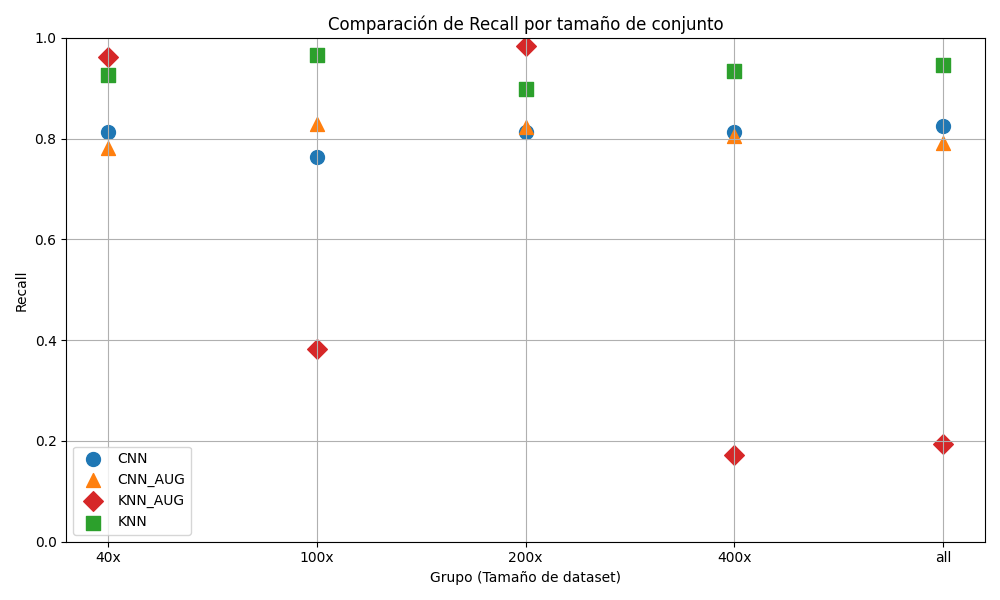
\includegraphics[width=\textwidth]{recall_comparativa_puntos.png}
        \caption{Comparación de Recall}
        \label{fig:figura8}
    \end{minipage}
    \hfill
    \begin{minipage}[b]{0.45\textwidth}
        \centering
        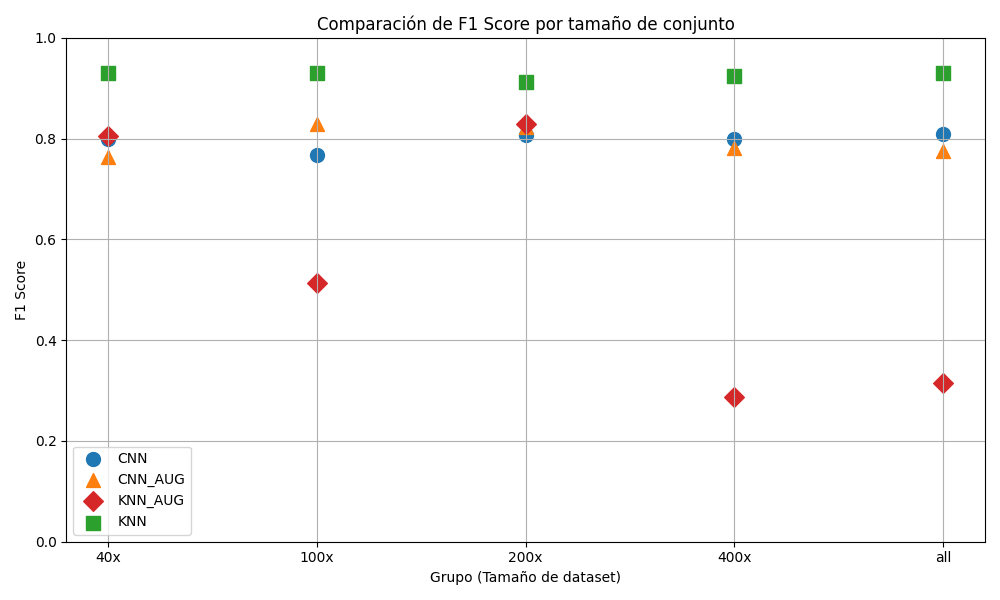
\includegraphics[width=\textwidth]{f1_score_comparativa_puntos.png}
        \caption{Comparación de F1 Score}
        \label{fig:figura9}
    \end{minipage}
\end{figure}

\newpage
En la presente experimentación, se evaluaron de manera sistemática los resultados obtenidos por los distintos modelos a través de dos tipos de representaciones gráficas. El primer conjunto de figuras (\ref{fig:figura1}, \ref{fig:figura2}, \ref{fig:figura3}, \ref{fig:figura4}, \ref{fig:figura5}) permite comparar las métricas clave de evaluación (Accuracy, F1 Score, Precision y Recall) entre los modelos entrenados sobre un mismo conjunto de datos, abarcando cinco configuraciones distintas según la magnificación de las imágenes. En estas comparaciones se incluyen cuatro variantes experimentales: CNN sin aumento de datos, para analizar su rendimiento sobre datos similares al entrenamiento; CNN con aumento, para evaluar su capacidad de adaptación ante transformaciones visuales; KNN sin aumento, que permite medir su rendimiento en un entorno cerrado; y KNN con aumento, que sirve para analizar su robustez ante variaciones visuales no vistas durante la generación del espacio latente.

El segundo conjunto de gráficas(\ref{fig:figura6}, \ref{fig:figura7}, \ref{fig:figura8}, \ref{fig:figura9}) invierte el enfoque, mostrando la evolución de una única métrica a través de todos los modelos disponibles, lo que facilita el análisis transversal del comportamiento de cada enfoque respecto a una métrica concreta. \\

De la interpretación de estas gráficas se desprenden varios aspectos relevantes: 

\begin{itemize}
    \item En primer lugar, se observa la notable estabilidad del modelo CNN, cuyas métricas se mantienen relativamente constantes independientemente del tamaño del conjunto de datos o de la magnificación, lo que indica una buena capacidad de generalización. Esto refuerza la idoneidad del modelo CNN en contextos clínicos donde la variabilidad de las muestras puede ser alta.
    \item En segundo lugar, se constata que el enfoque basado en autoencoder + KNN obtiene un rendimiento superior al del modelo CNN cuando se trabaja sobre datos no aumentados, lo que sugiere una gran eficacia del sistema en contextos cerrados o controlados. Sin embargo, esta ventaja desaparece bruscamente al aplicar técnicas de data augmentation. Las métricas del KNN se degradan significativamente en presencia de transformaciones geométricas o visuales, revelando una importante fragilidad del sistema ante cambios en los datos de entrada.
\end{itemize}

Esta degradación se atribuye a la alteración de los vectores latentes generados por el autoencoder cuando se introducen variaciones visuales, ya que al introducir cambios visuales el vector latente a analizar por el KNN es distinto al vector original por lo que puede dar otro valor de clasificación. A diferencia de la CNN, que ajusta sus parámetros internos durante el entrenamiento para acomodar estas variaciones, el sistema basado en KNN no posee un mecanismo de adaptación, lo que conduce a una pérdida de coherencia en el espacio latente y, por ende, a un descenso en la precisión de la clasificación.\\

\section{Manual de usuario}

Esta herramienta permite cargar una imagen desde el dispositivo y realizar un análisis para determinar si corresponde a un caso \textbf{benigno} o \textbf{maligno}. Los pasos a seguir son los siguientes:
\newpage

\subsection*{Paso 1: Seleccionar una Imagen}

\textbf{Opción 1: Cargar por Ruta}
\begin{itemize}
    \item Haz clic en el botón \textbf{Seleccionar Imágenes}.
    \item Navega por tus carpetas y selecciona las imágenes que deseas analizar.
    \item Las imágenes seleccionadas aparecerán en el panel de previsualización.
    \begin{figure}[!ht]
        \centering
        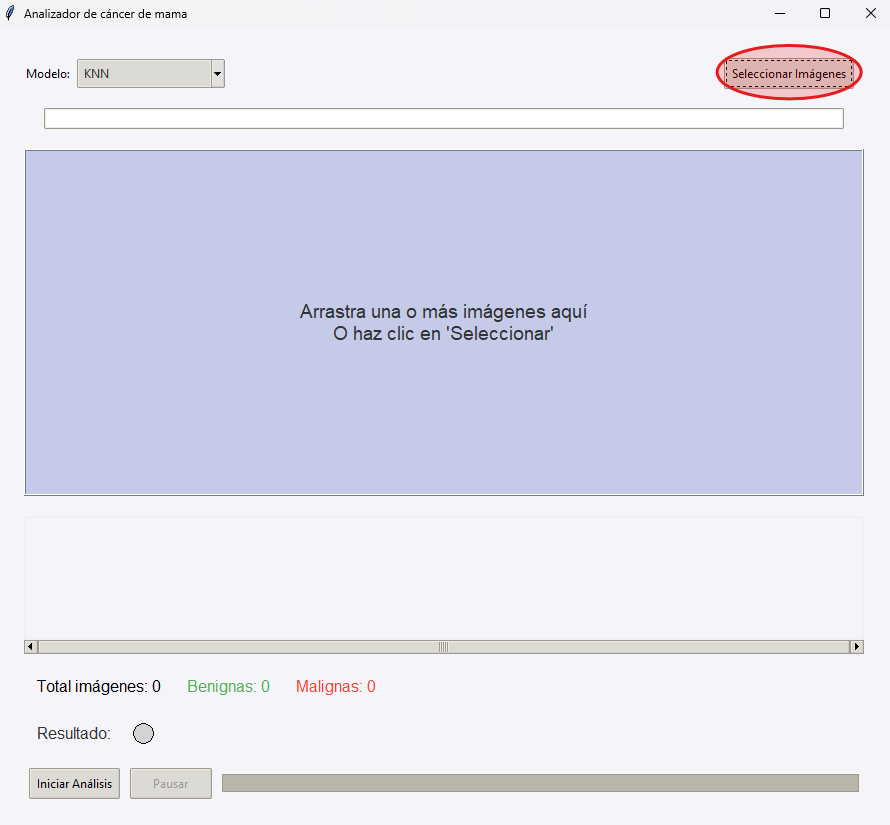
\includegraphics[width=0.4\textwidth]{CargarRuta.png}
        \caption{Botón para la carga de imágenes}
        \label{fig:imagen_carga}
    \end{figure}
\end{itemize}

\textbf{Opción 2: Arrastrar y Soltar}
\begin{itemize}
    \item Puedes arrastrar la imagen directamente desde tu explorador de archivos y soltarla en el área indicada de la aplicación.
    \item Las imágenes se cargarán automáticamente en la aplicación.
    \begin{figure}[!ht]
        \centering
        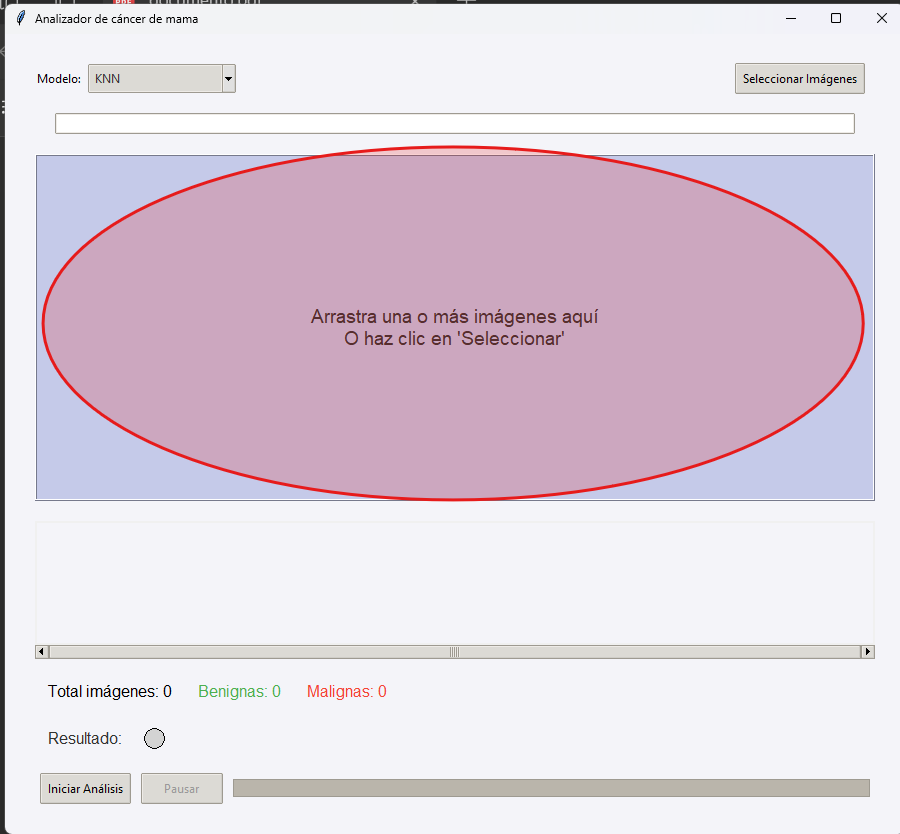
\includegraphics[width=0.4\textwidth]{ArrastrarySoltar.png}
        \caption{Pantalla de carga de imágenes}
        \label{fig:imagen_carga_arrastrar}
    \end{figure}
\end{itemize}

\newpage
\subsection*{Paso 2: Seleccionar el Modelo}

\begin{itemize}
    \item Una vez que hayas cargado la imagen correctamente, tiene que seleccionar el modelo.
    \item Arriba a la izquierda de la pantalla, verás un menú desplegable con las opciones de modelos disponibles.
    \begin{figure}[!ht]
        \centering
        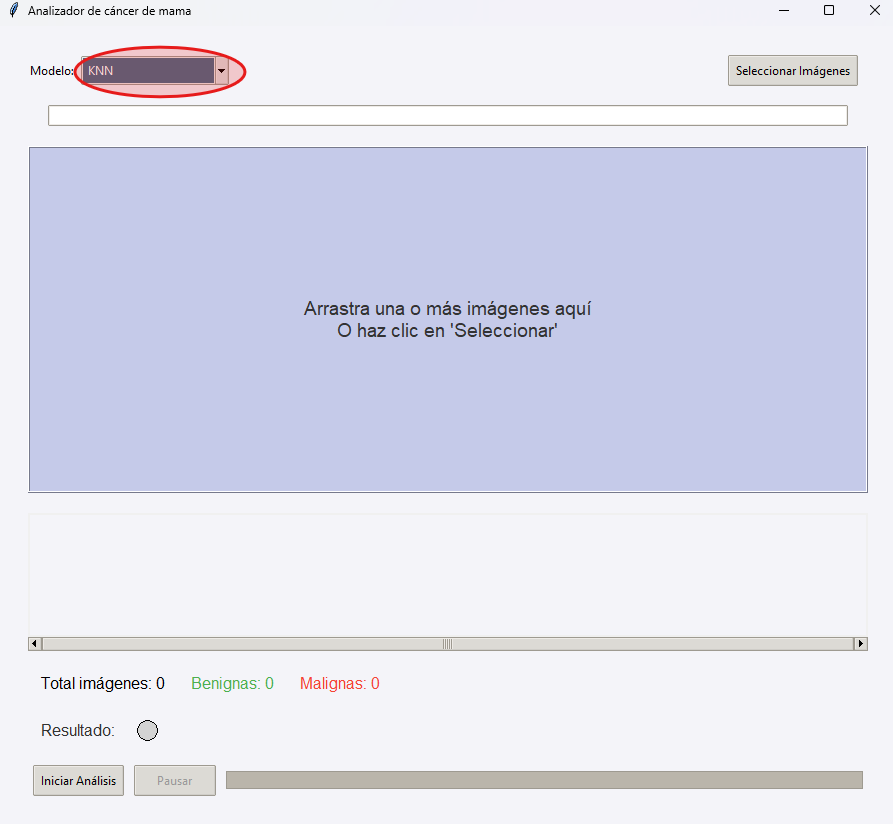
\includegraphics[width=0.4\textwidth]{SeleccionarModelo.png}
        \caption{Menú desplegable para seleccionar el modelo}
        \label{fig:seleccionar_imagen}
    \end{figure}
\end{itemize}

\subsection*{Paso 3: Iniciar el Análisis}

\begin{itemize}
    \item Una vez que hayas cargado la imagen correctamente, haz clic en el botón \textbf{Analizar}.
    \item La aplicación procesará la imagen y mostrará si corresponde a un caso maligno o benigno.
    \begin{figure}[!ht]
        \centering
        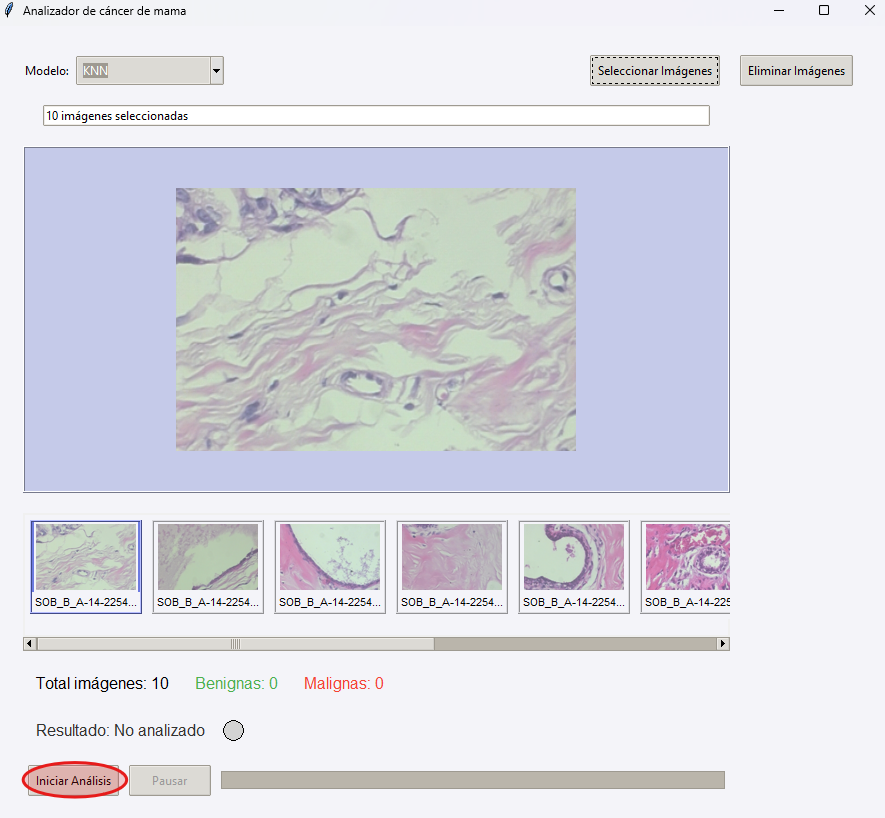
\includegraphics[width=0.4\textwidth]{IniciarAnalisis.png}
        \caption{Botón para iniciar el análisis}
        \label{fig:iniciar_analisis}
    \end{figure}
\end{itemize}
\newpage
\textbf{Otras opciones:}
\begin{itemize}
    \item Puedes pausar el análisis en cualquier momento haciendo clic en el botón \textbf{Pausar}.
    \begin{figure}[!ht]
        \centering
        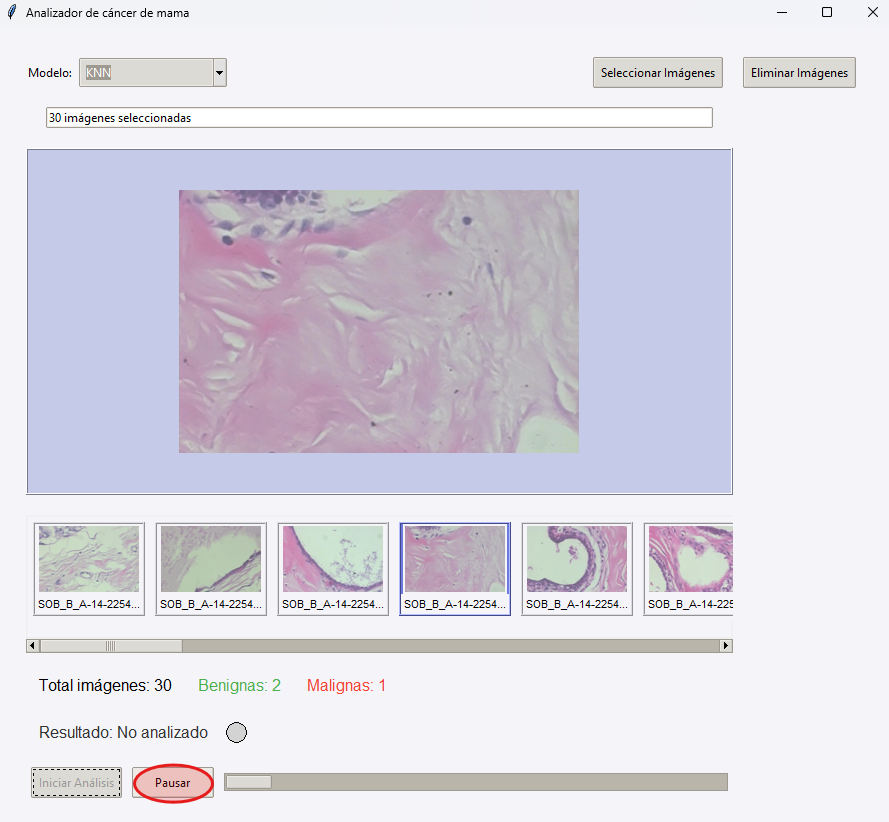
\includegraphics[width=0.4\textwidth]{PausarAnalisis.png}
        \caption{Botón para pausar el análisis}
        \label{fig:pausar_analisis}
    \end{figure}
    \item O si bien lo desea puede reanudar el análisis haciendo clic en el botón \textbf{Reanudar}.
    \begin{figure}[!ht]
        \centering
        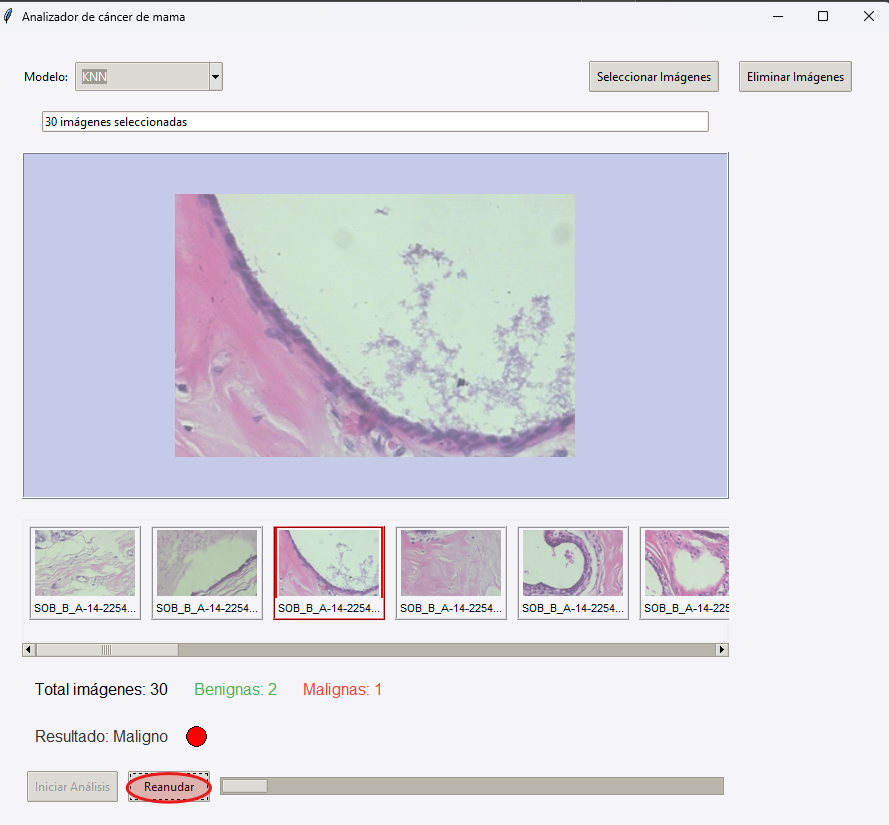
\includegraphics[width=0.4\textwidth]{ReanudarAnalisis.png}
        \caption{Botón para reanudar el análisis}
        \label{fig:reanudar_analisis}
    \end{figure}
\end{itemize}

\subsection*{Paso 4: Ver el Resultado}

\begin{itemize}
    \item Después de un breve momento, se mostrará el resultado en pantalla.
    \item Si la imagen es \textbf{benigna}, se mostrará un mensaje y un círculo indicador en color \textcolor{green}{verde}.
    \item Si la imagen es \textbf{maligna}, se mostrará un mensaje y un círculo indicador en color \textcolor{red}{rojo}.
    \begin{figure}[!ht]
        \centering
        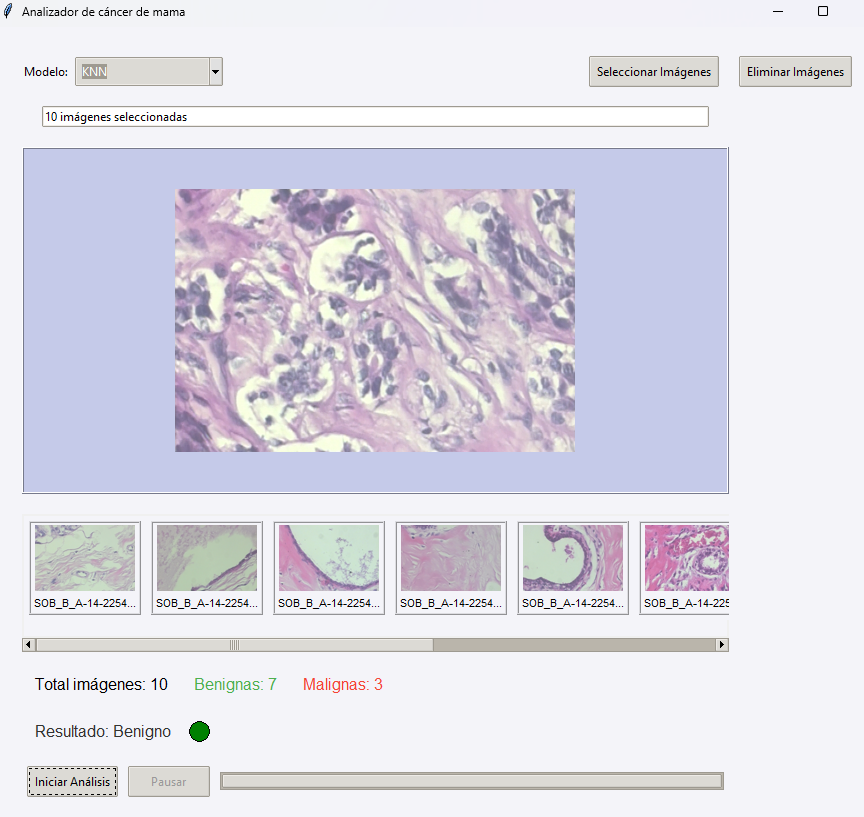
\includegraphics[width=0.4\textwidth]{Ver el Resultado.png}
        \caption{Pantalla de resultado del análisis}
        \label{fig:resultado}
    \end{figure}
\end{itemize}

\subsection*{Paso 5: Realizar Nuevos Análisis}

\begin{itemize}
    \item Puede eliminar los resultados dados haciendo clic al boton de \textbf{Eliminar} o bien puede volver a cargar otras imágenes haciendo clic nuevamente en el botón \textbf{Seleccionar} o arrastrándolas directamente.
    \item El proceso de análisis es el mismo para cada imagen que cargues.
    \begin{figure}[!ht]
        \centering
        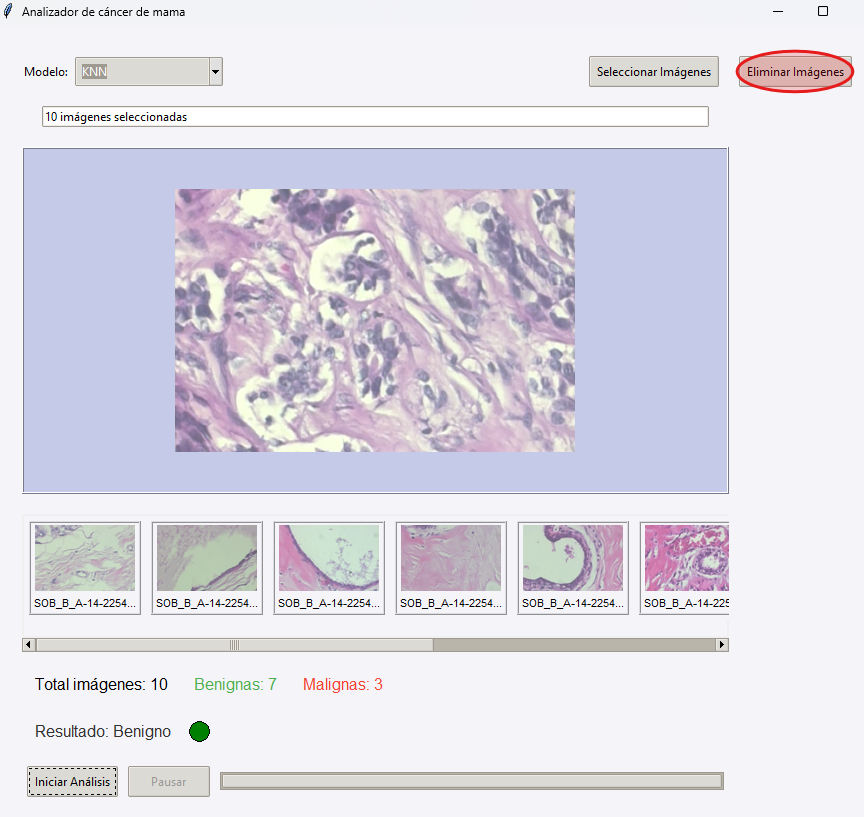
\includegraphics[width=0.4\textwidth]{EliminarImagenes.png}
        \caption{Botón para eliminar imágenes}
        \label{fig:eliminar_imagenes}
    \end{figure}
\end{itemize}

\newpage
\section{Conclusiones}
Este trabajo ha comparado \textit{dos enfoques} para la clasificación de imágenes histológicas de cáncer de mama: un modelo de red neuronal convolucional (\textbf{CNN}) entrenado de forma supervisada, y un sistema basado en autoencoders convolucionales combinados con el algoritmo k-Nearest Neighbors (\textbf{KNN}).\\

El modelo CNN ha demostrado ser robusto, estable y eficaz, alcanzando hasta un 82.8\% de precisión con técnicas de \textit{data augmentation}. Esta capacidad de adaptarse a variaciones visuales como cambios en iluminación, orientación o resolución lo hace especialmente adecuado para su uso en situaciones reales, donde las imágenes histológicas pueden variar sustancialmente según el paciente, el escáner o el protocolo de adquisición. Además, su rendimiento ha sido consistente a través de diferentes magnificaciones y configuraciones de entrenamiento, lo que refuerza su fiabilidad como herramienta de soporte en entornos clínicos.\\

En contraste, el enfoque con autoencoder y KNN mostró un rendimiento excelente en condiciones controladas, llegando hasta un 90.1\% de precisión cuando los datos de prueba eran similares a los de entrenamiento. Sin embargo, su desempeño se degradó de forma significativa al introducir transformaciones visuales, con caídas abruptas en precisión y otras métricas clave. Este fenómeno se explica por el cambio en los vectores latentes generados por el autoencoder cuando se alteran visualmente las imágenes debido a que los cambios visuales alteran los vectores latentes del autoencoder, y al depender de un clasificador externo como KNN, sin capacidad de adaptación, se pierde coherencia y se reduce la fiabilidad del sistema.\\

Este comportamiento expone una limitación crítica del método KNN en contextos médicos: la falta de adaptabilidad ante datos no vistos o alterados, lo que puede traducirse en errores diagnósticos si no se gestiona adecuadamente. En un entorno médico, donde las decisiones automáticas pueden tener implicaciones directas sobre la vida del paciente, es indispensable contar con modelos que no solo ofrezcan buenas métricas en laboratorio, sino que mantengan su rendimiento ante variaciones reales y potencialmente imprevistas.\\

Por tanto, el modelo CNN se perfila como la opción más adecuada para aplicaciones clínicas, ofreciendo un balance óptimo entre rendimiento, robustez y adaptabilidad. El enfoque con KNN, si bien limitado para clasificación directa en entornos abiertos, podría seguir siendo útil en tareas complementarias como la recuperación de imágenes similares, la búsqueda por contenido o como sistema de apoyo en análisis exploratorios.

\newpage
\section{Autoevaluación de cada miembro del equipo}
\renewcommand{\tablename}{Tabla}

\begin{table}[!ht]
\centering
\renewcommand{\arraystretch}{1.5}
\setlength{\tabcolsep}{6pt}
\resizebox{\textwidth}{!}{ % Ajusta automáticamente al ancho
\begin{tabular}{|p{3.5cm}|p{5cm}|c|c|c|} % Ajusté el ancho de la primera columna
\hline
\multicolumn{2}{|c|}{\multirow{2}{*}{\textbf{\small Secciones}}} & \multicolumn{3}{c|}{\textbf{Nombre}} \\ \cline{3-5}
\multicolumn{2}{|c|}{} & \textbf{\footnotesize Lucas M. Herencia Solís} & \textbf{\footnotesize Marina Calero López} & \textbf{\footnotesize Juan A. Moreno Moguel} \\ \hline

\multirow{3}{*}{\makecell{\textbf{\small Exposición}}} 
    & Compresión y dominio & Excelente & Regular & Bien \\ \cline{2-5}
    & Exposición didáctica & Excelente & Bien & Excelente \\ \cline{2-5}
    & Integración equipo & Excelente & Excelente & Excelente \\ \hline

\multirow{3}{*}{\makecell{\textbf{\small Implementación}}} 
    & Objetivos & Excelente & Bien & Bien \\ \cline{2-5}
    & Aspectos didácticos & Excelente & Bien & Bien \\ \cline{2-5}
    & Experimentación y conclusión & Excelente & Excelente & Bien \\ \hline

\multirow{3}{*}{\makecell{\textbf{\small Documentación}}} 
    & Contenidos & Excelente & Bien & Bien \\ \cline{2-5}
    & Divulgación de contenidos & Excelente & Excelente & Excelente \\ \cline{2-5}
    & Bibliografía / Recursos científicos & Excelente & Excelente & Excelente \\ \hline
\end{tabular}
}
\caption{Evaluación del desempeño por secciones}
\label{tab:evaluacion}
\end{table}


\section{Tabla de tiempos}
A continuación se presenta la tabla de tiempos dedicados por cada miembro del equipo a lo largo del desarrollo del proyecto.\\

Primero se pondrá una tabla resumen con el tiempo total dedicado por cada miembro del equipo a dicha tarea en especifico, y posteriormente se incluirán los informes de cada uno de los miembros del equipo de manera más detalla y con la descripción clara de dicha tarea.\\

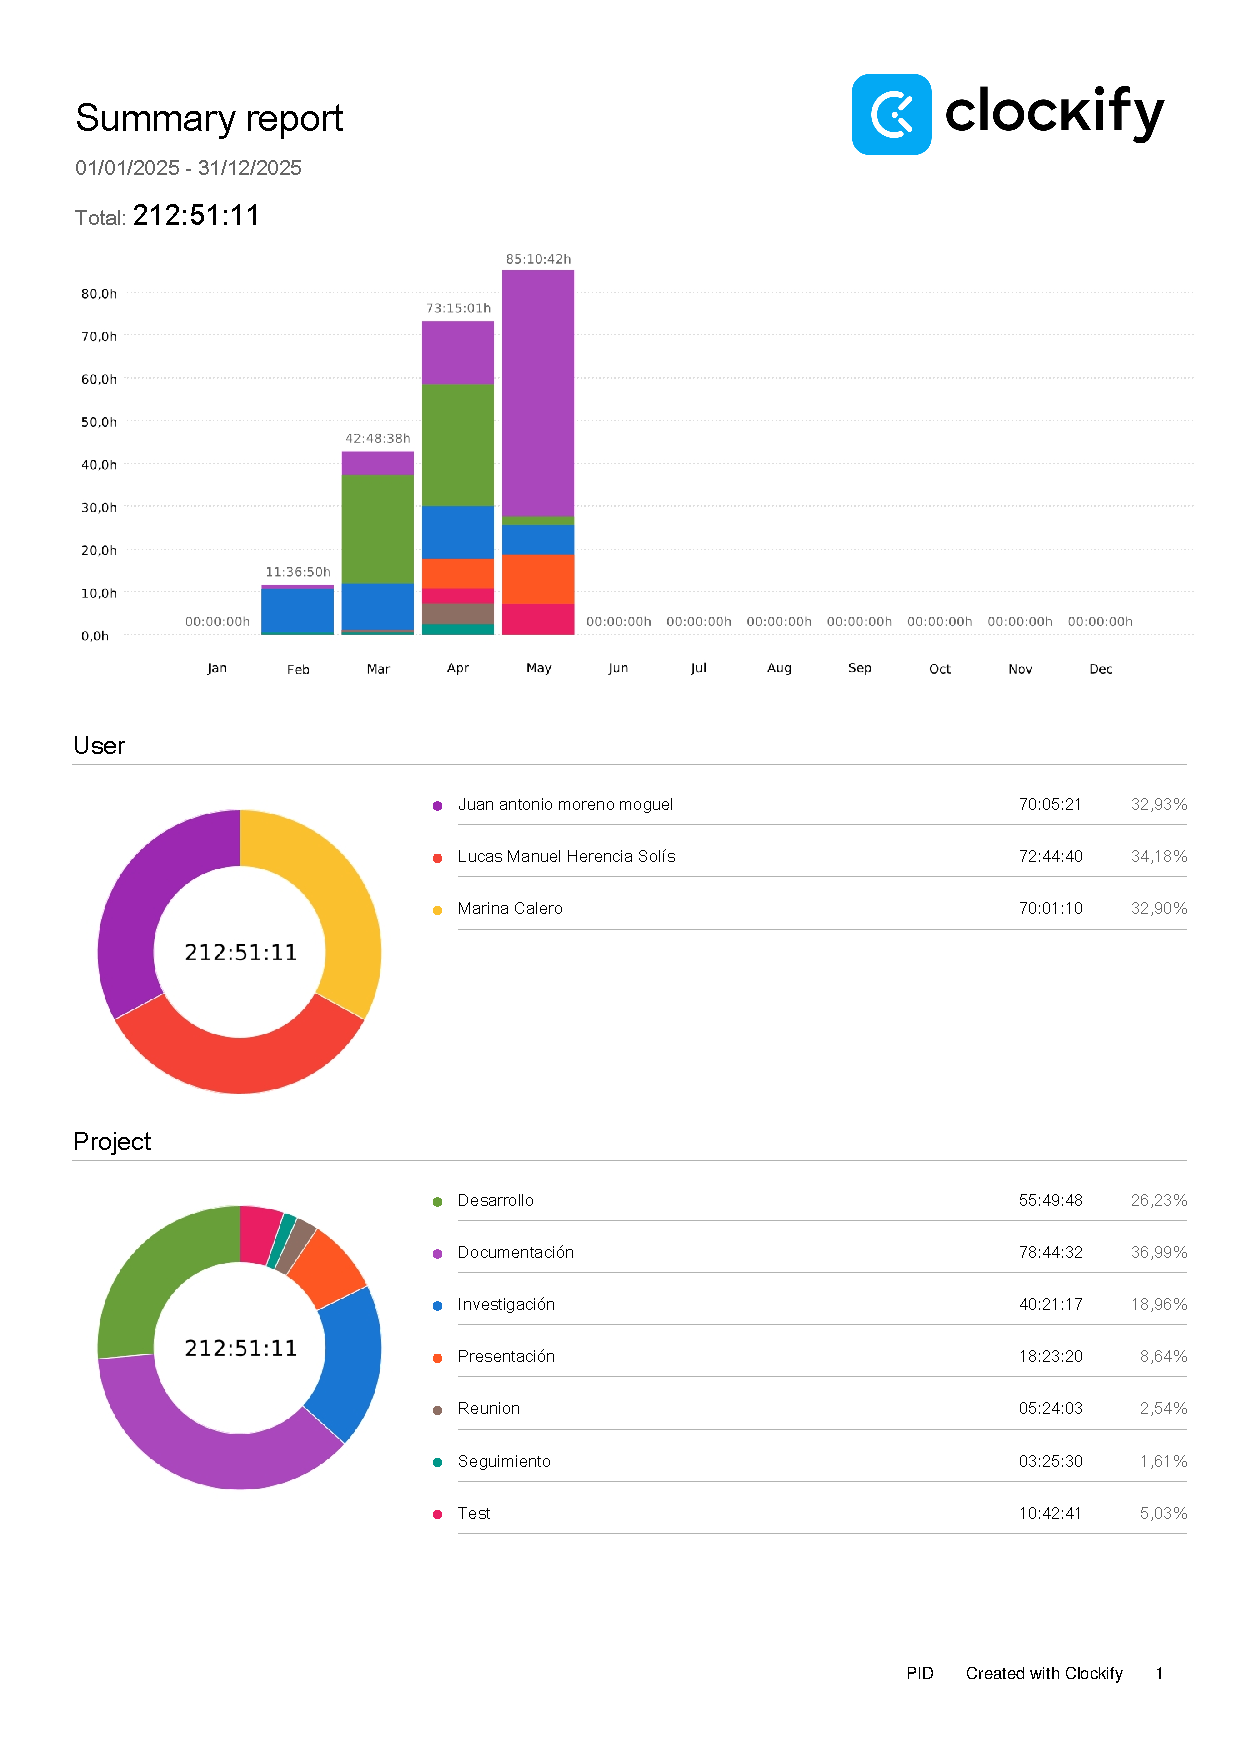
\includepdf[pages=-]{Clockify_Time_Report_Summary_01_01_2025-31_12_2025.pdf}  

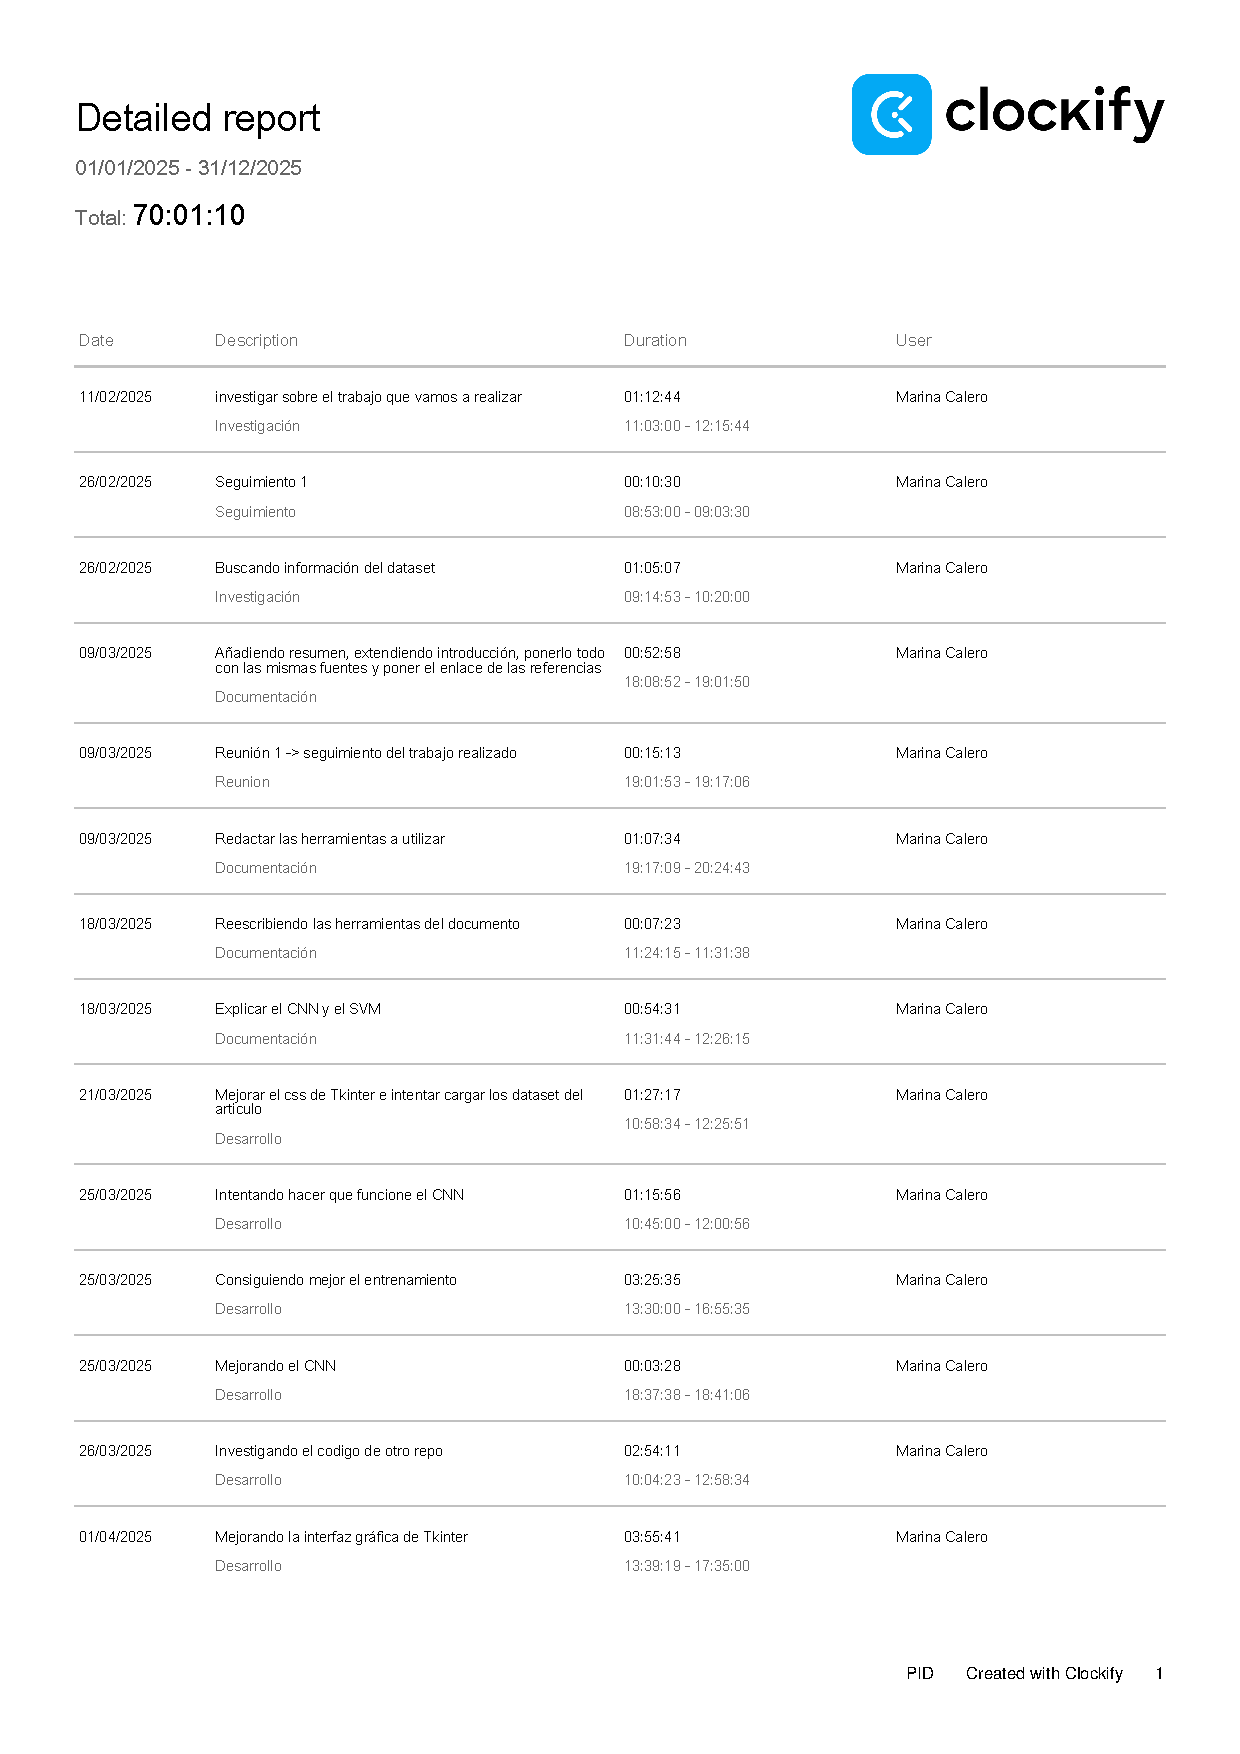
\includepdf[pages=-]{marinaclockify.pdf}  
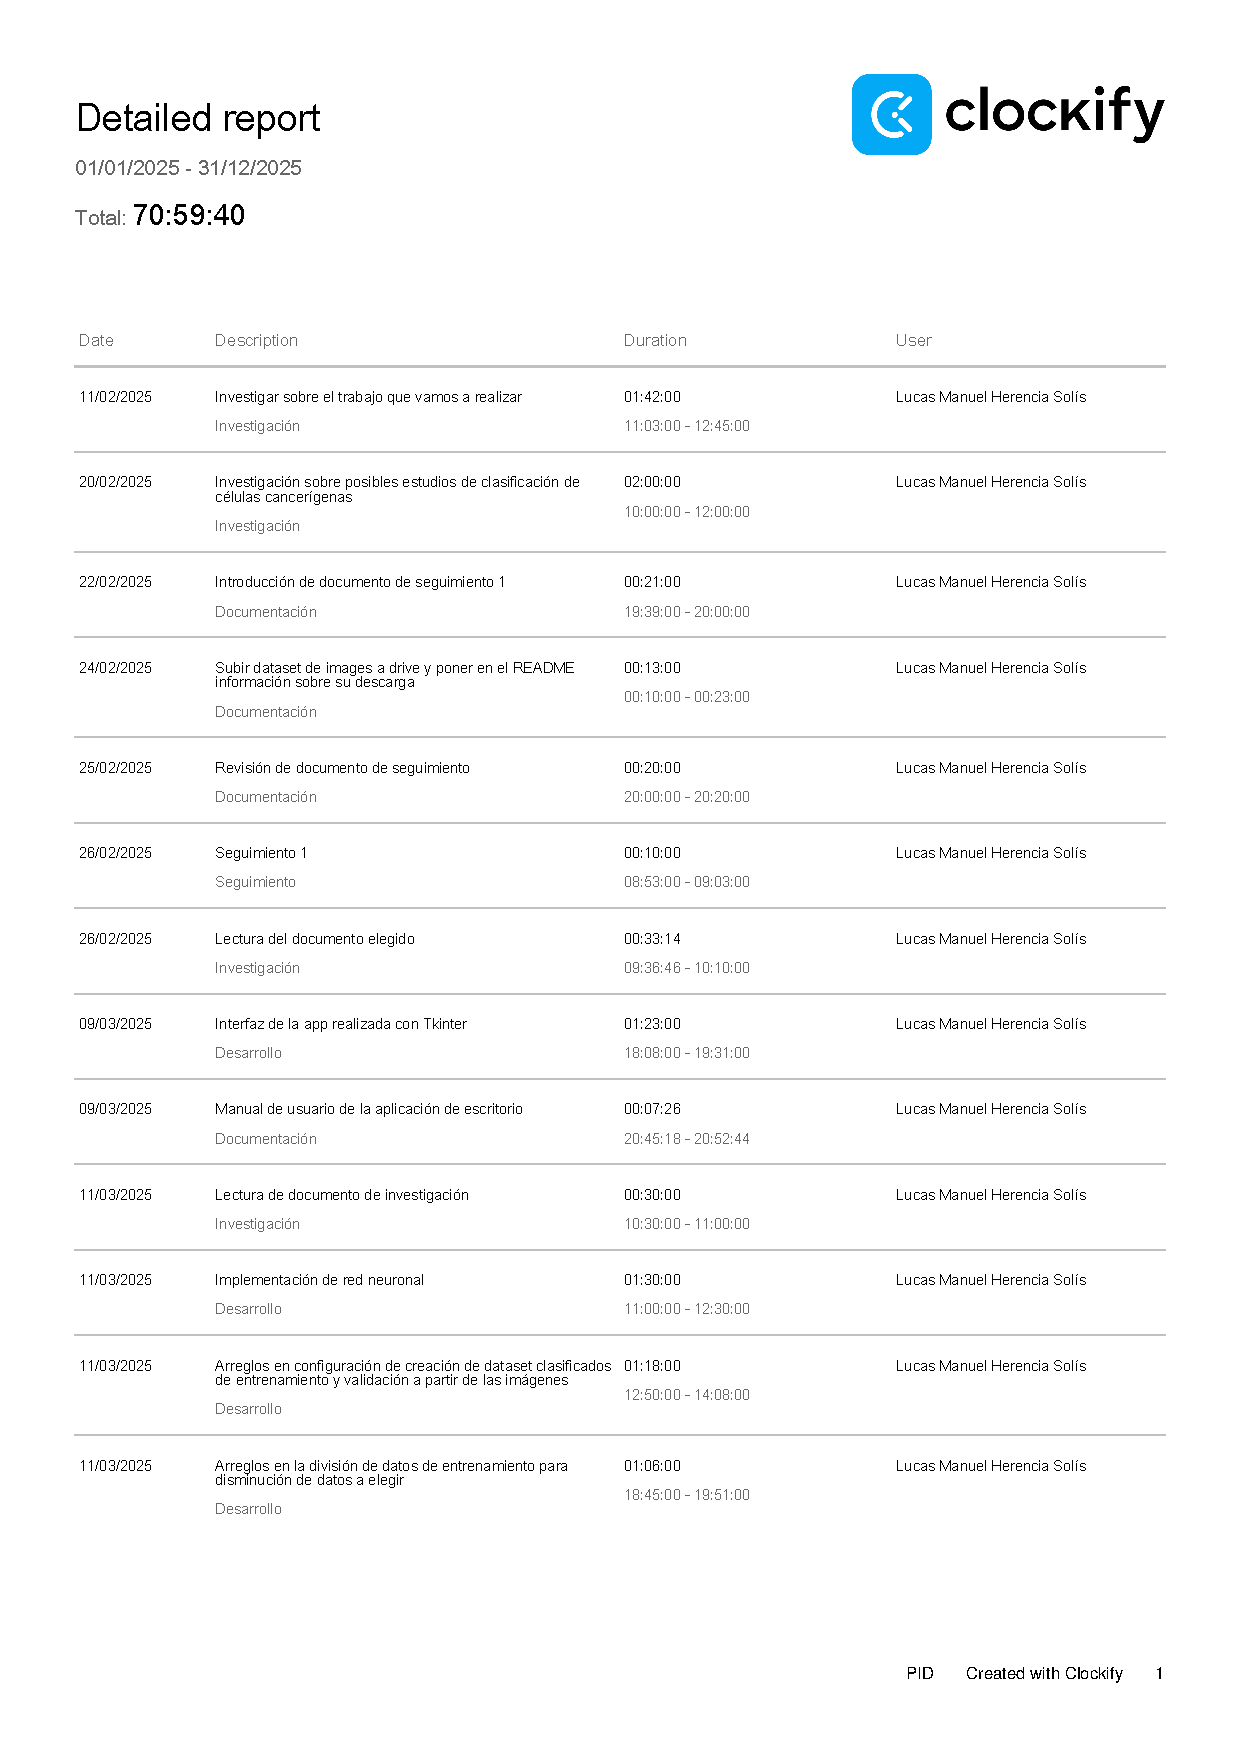
\includepdf[pages=-]{lucasclockify.pdf}
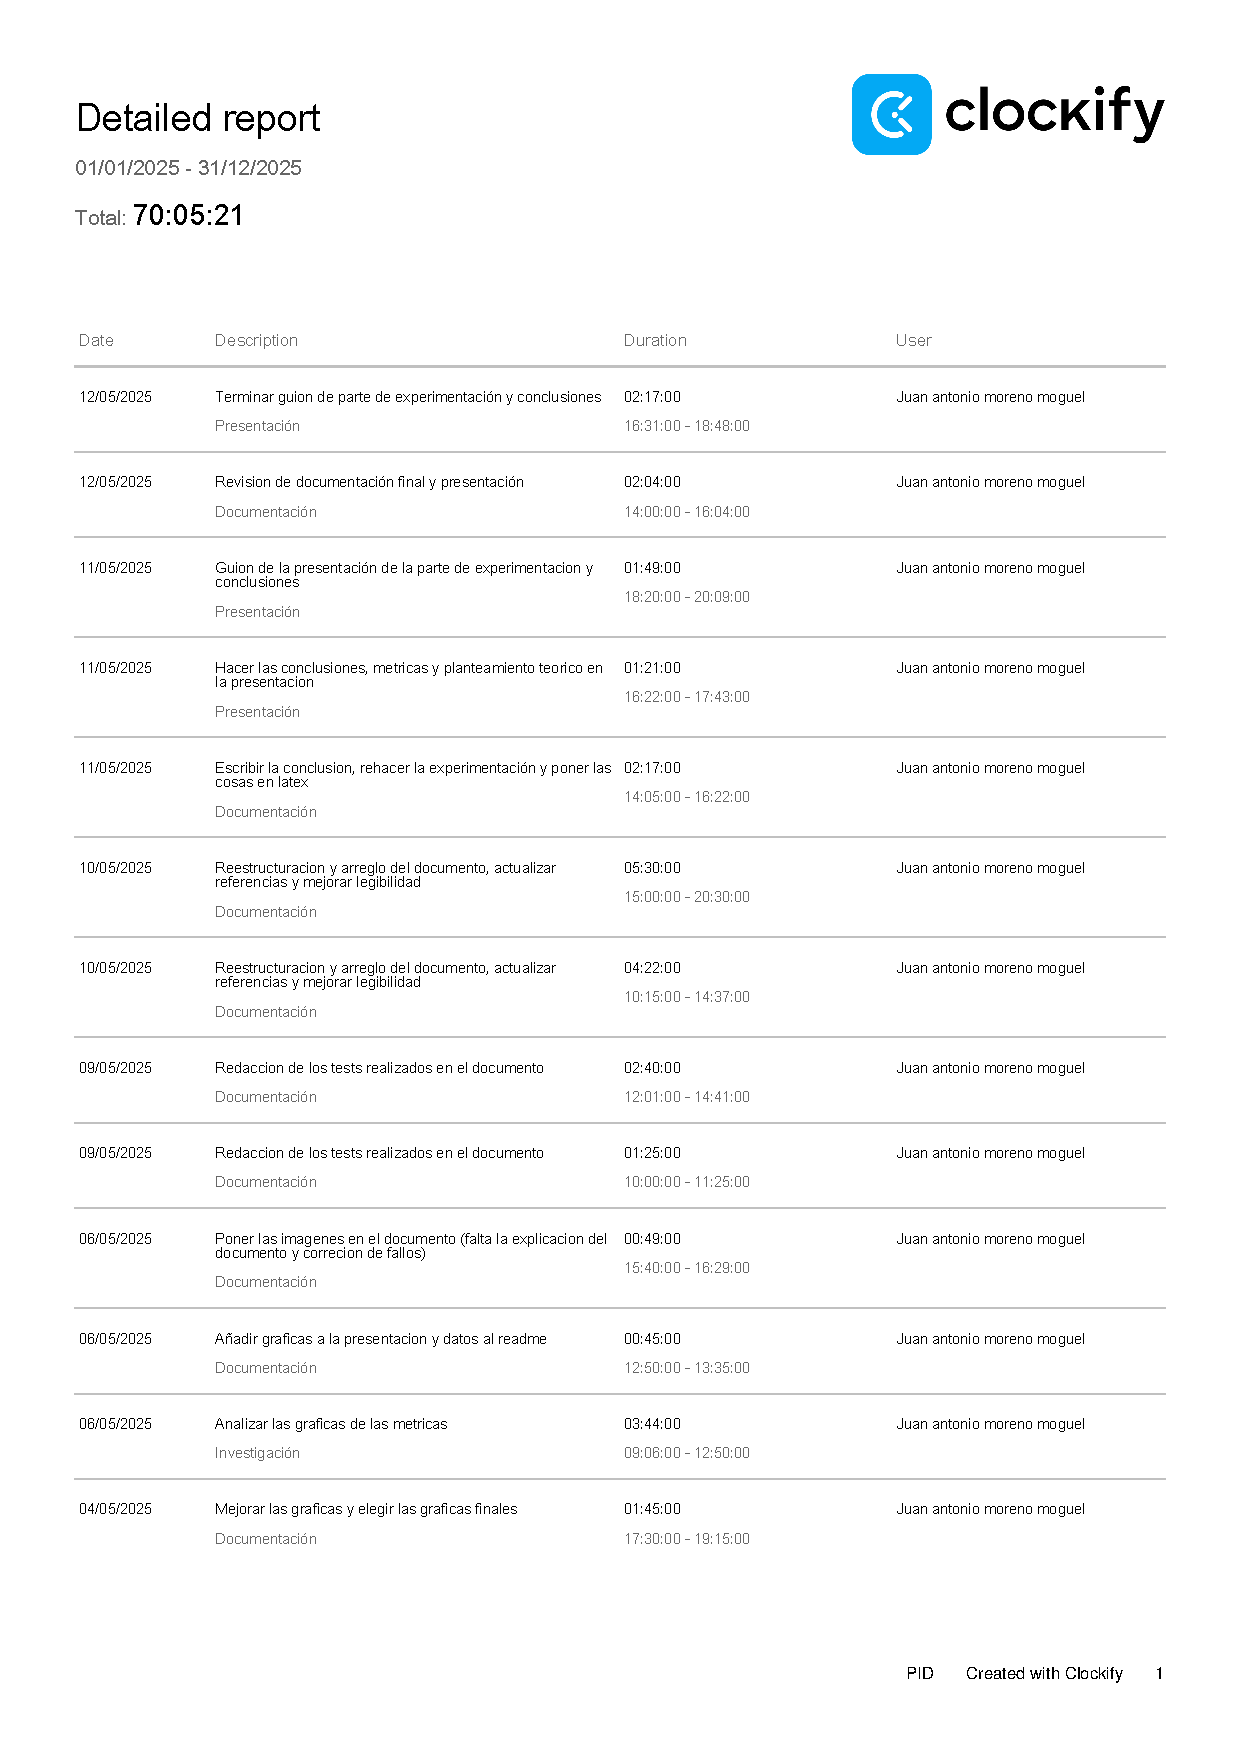
\includepdf[pages=-]{juanclockify.pdf}

\newpage
\addcontentsline{toc}{section}{Bibliografía} 
\printbibliography

\end{document}
